\documentclass[10pt]{article}
\usepackage[utf8]{inputenc}
\usepackage[T1]{fontenc}
\usepackage{amsmath}
\usepackage{amsfonts}
\usepackage{amssymb}
\usepackage[version=4]{mhchem}
\usepackage{stmaryrd}
\usepackage{graphicx}
\usepackage[export]{adjustbox}
\graphicspath{ {./images/} }
\usepackage{hyperref}
\hypersetup{colorlinks=true, linkcolor=blue, filecolor=magenta, urlcolor=cyan,}
\urlstyle{same}

\title{StreamPIM: Streaming Matrix Computation in Racetrack Memory }


\author{Yuda An $^{* 1}$, Yunxiao Tang ${ }^{* 1}$, Shushu Yi $^{1}$, Li Peng ${ }^{1}$, Xiurui Pan ${ }^{1}$\\
Guangyu Sun ${ }^{1,3}$, Zhaochu Luo ${ }^{1}$, Qiao Li $^{2}$, Jie Zhang ${ }^{1}$\\
Computer Hardware and System Evolution Laboratory,\\
Peking University ${ }^{1}$, Xiamen University ${ }^{2}$,\\
Beijing Advanced Innovation Center for Integrated Circuits 3\\
https://www.chaselab.wiki}
\date{}


\begin{document}
\maketitle


\begin{abstract}
Racetrack memory (RM) techniques have become promising solutions to resolve the memory wall issue as they increase memory density, reduce energy consumption and are capable of building processing-in-memory (PIM) architectures. RM can place arithmetic logic units in or near its memory arrays to process tasks offloaded by the host. While there already exist multiple studies of processing in RM, these solutions, unfortunately, suffer from data transfer overheads imposed by the loose coupling of the memory core and the computation units. To address this issue, we propose StreamPIM, a new processing-in-RM architecture, which tightly couples the memory core and the computation units. Specifically, StreamPIM directly constructs a matrix processor from domain-wall nanowires without the usage of CMOS-based computation units. It also designs a domainwall nanowire-based bus, which can eliminate electromagnetic conversion. StreamPIM further optimizes the performance by leveraging RM internal parallelism. Our evaluation results show that StreamPIM achieves $39.1 \times$ higher performance and saves $58.4 \times$ energy consumption, compared with the traditional computing platform.
\end{abstract}

\section*{I. Introduction}
Over the last decade, emerging large-scale applications, such as machine learning, scientific computing and graph analysis [23], [28], [42], [50], have received a considerable attention owing to their impacts on a wide range of research and industry domains [3], [60], [67]. Compared to the traditional ones, these applications are both data-intensive and computeintensive. This is because such applications commonly require massive matrix computations, which consume a huge amount of memory to store all the elements of the matrices and need a huge amount of computing power. For instance, a popular machine learning model, GPT-3 [11], has 175 billion parameters, which takes up to $800 \mathrm{~GB}$ of memory and 34 -day computing in a 1024-node cluster [51]. The state-of-the-art language model, GPT-4 [55], is reported to have even more parameters, consuming more memory and power.

The continuous development of large-scale applications stimulates increasing demands for larger memory capacities and higher computing power [33], [74]. Unfortunately, the existing computing systems have not kept up with the quick development of large-scale applications for two reasons. Firstly,

\begin{itemize}
  \item These authors contributed equally to this work and should be considered co-first authors.
\end{itemize}

\begin{center}
\begin{tabular}{|c|c|c|c|c|c|}
\hline
Memory & Access & Density & Energy & Reliability & PIM integration \\
\hline
DRAM & fast & low & high & high & CMOS [64] \\
\hline
PCRAM & slow & high & low & low & CMOS [43] \\
\hline
ReRAM & slow & high & low & low & in-cell [14] \\
\hline
MRAM & fast & low & low & high & \begin{tabular}{c}
CMOS [31] \\
in-cell [19] \\
\end{tabular} \\
\hline
RM & fast & high & low & high & \begin{tabular}{c}
CMOS [53] \\
skyrmion [45] \\
\end{tabular} \\
\hline
\end{tabular}
\end{center}

TABLE I: Comparison of different memory techniques.

the traditional memory system is built from DRAM, which faces multiple challenges in scaling its technology down. Specifically, DRAM has the limitations of retention time violations, insufficient sensing margins, and low-reliability issues [30], [36], [37], [48]. Secondly, the Von Neumann architecture [7], which has been widely adopted by the computing systems, suffers from the huge overheads imposed by data movements. For example, researches [13], [24] reveal that moving data from the memory to the processor consumes $3 \times \sim 11 \times$ more energy than data processing in the processor.

Non-Volatile Memory (NVM) [18], [58] has become a promising candidate to replace DRAM as the main memory. NVM can deliver much higher memory density than DRAM. It also supports process-in-memory (PIM) techniques [14], [31], [43] to enable parallel matrix computation within memory, which can eliminate the data movement overheads. Table I summarizes the key features of different NVM solutions. While Resistive Random Access Memory (ReRAM) [40], [79] outperforms DRAM in terms of memory density and energy consumption, ReRAM is vulnerable to reliability issues owing to its error-prone intrinsic [39]. Phase Change Random Access Memory (PCRAM) [12], [62] can address the reliability issues, but has a much longer access latency than DRAM. SpinTransfer Torque Magnetic Random Access Memory (STTMRAM) [17], [25] can achieve shorter latency than DRAM. Unfortunately, STT-MRAM suffers from a low memory density, making it difficult to replace DRAM directly. Domain-Wall Memory (DWM) [26], [57], also referred to as Racetrack Memory (RM), achieves a good balance among the requirements of performance, energy, density, and reliability (cf. Table I).

Multiple studies have explored the design spaces for processing matrix computations within RM [45], [53], [80]. SPIM [45] proposes to integrate multiple skyrmion-based computation\\
units in the RM, each processing the data stored in adjacent memory cores. DW-NN [80], in contrast, employs alternative computation units based on CMOS, which is more practical in device fabrication. CORUSCANT [53], the state-of-the-art process-in-RM work, also employs CMOS-based computation units. It leverages a mechanism called Transverse Read [63] to achieve lower computation latency and higher reliability. However, despite the benefits of PIM, computation units in prior works require iteratively loading data from the memory cores and storing back intermediate results, which incurs data conversion overheads (e.g., electromagnetic conversion). Considering that the write latency and power of RM are relatively high [82], the prior approaches suffer from such conversion overheads. To quantitatively analyze how the intensive memory accesses can affect the overall performance, we perform a breakdown analysis of execution time and energy consumption in CORUSCANT by examining various types of arithmetic operations (cf. Figure 4 for details). Transferring data between the RM array and the computation units accounts for $69 \%$ and $70 \%$ of the total execution time and energy consumption, respectively.

To tackle the aforementioned challenges, we propose a new architecture for process-in-RM, called StreamPIM, which leverages the unique shift operation of RM to eliminate the data conversion overheads imposed by traditional read and write operations between computation units and memory arrays. Specifically, StreamPIM directly constructs a matrix processor from domain-wall nanowires ( $R M$ Processor) which performs computation with shift operations without the usage of CMOS-based computation units. Unlike traditional computation units, which are designed for scalar operations, the RM processor is well-customized for complex matrix computations, eliminating unnecessary intermediate results. To improve the efficiency of data migration within RM, StreamPIM proposes a domain-wall nanowire based bus ( $R M$ Bus). This new bus directly transfers data with shift operations, avoiding electromagnetic conversion. StreamPIM further accelerates the matrix processing by exploiting the internal parallelism in RM and streaming the data transfer and data processing via a pipelined manner. For matrix computation benchmarks and end-to-end applications, our evaluation shows that StreamPIM respectively achieves $39.1 \times$ and $29.63 \times$ average performance improvement compared to traditional computing system.

Our contributions are summarized as follows:

\begin{itemize}
  \item New process-in-RM architecture for stream processing: We propose a new process-in-RM architecture, in which both the computation units and the RM internal buses are built entirely from domain-wall nanowires. By doing so, StreamPIM performs both the computation and the data transfer via simple RM shift operations without electromagnetic conversion, thereby eliminating the RM access overheads. In addition, since StreamPIM only uses shift operations, data can be moved and processed in a streaming fashion, improving system throughput. - Customized RM processor design for matrix computations: The computation units in the traditional PIM support only a few types of simple arithmetical operations. They generate massive intermediate results during a large-scale matrix computation, which introduces frequent RM accesses. In contrast, we design a customized RM processor to execute the entire matrix computation in a streaming fashion. Our RM processor conducts various vector operations, such as addition, scalarvector multiplication, and dot product, by leveraging the FanOut mechanism [71] and Domain-Wall Diode [47].

  \item Domain-wall nanowire based bus design: To mitigate the data transfer overheads imposed by electromagnetic conversion, our StreamPIM replaces the electrical-based bus with a new type of bus based on domain-wall nanowires. The data transfers are thus performed by shift operations on domainwall nanowires. However, owing to the intrinsic nature of domain-wall nanowires, this new design suffers from three main limitations: (1) the uncertainty of transfer length; (2) the low throughput due to high latency; (3) the shift fault problem due to long distance. To overcome these challenges, we propose to divide the new bus into segments of the same length. At every clock cycle, the data in the bus are shifted over the length of one segment, ensuring constant transfer length.

  \item Architecture design for parallel matrix processing: We introduce a cross-layer design to utilize RM internal parallelism better. Specifically, the RM processors are integrated in each memory array, bringing hardware parallelism to the subarray level. The matrix representation and placement are carefully designed to exploit hardware parallelism from the software aspect. Lastly, the essential data copy and preparation in matrix operations are decoupled from the explicit computation, resolving the blocking issue between RM read/write and shift operations for parallelism exploration.

\end{itemize}

\section*{II. BACKGROUND}
\section*{A. Internal Architecture of $R M$}
Memory core. Domain-Wall Memory (DWM), or Racetrack Memory (RM), is a new type of spintronic-based non-volatile memory technique [56], [72]. We will use DWM and RM interchangeably in this paper. An RM primarily consists of multiple domain-wall (ferromagnetic) nanowires, which are also called racetracks in prior works. Figure 1 shows the core structure of a domain-wall nanowire, which consists of multiple domains separated by domain-walls. Each domain stores onebit data, whose value is determined by the magnetization direction. Thus, a domain-wall nanowire is capable of storing multiple bits. A domain-wall nanowire contains one or multiple access ports to perform read and write operations. An access port is a ferromagnetic component with a fixed reference magnetization direction. A domain and an access port together form a Magnetic Tunnel Junction (MTJ) structure. To read data from a domain, a read voltage is applied to the MTJ. The comparison of the magnetization directions between the target domain and the reference determines the magneto resistance of the MTJ. The read operation leverages this feature to sense out the bit value. To write a domain is to apply a high write current across MTJ, which can change the magnetization direction of the target domain. Thus, RM write latency and energy are much higher than those of RM read operations. Considering

\begin{center}
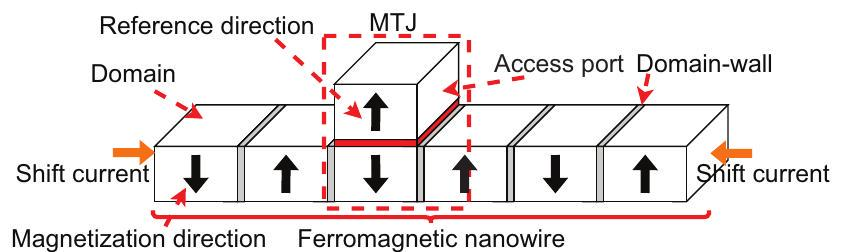
\includegraphics[max width=\textwidth]{2024_05_12_abeba8a85da5b5ec4c7bg-03(1)}
\end{center}

Fig. 1: Core structure of a domain-wall nanowire.

\begin{center}
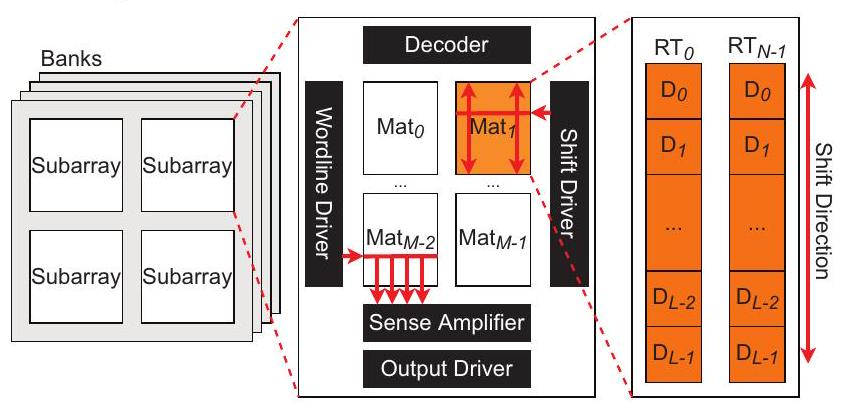
\includegraphics[max width=\textwidth]{2024_05_12_abeba8a85da5b5ec4c7bg-03(5)}
\end{center}

Fig. 2: Typical architecture of racetrack memory.

the cost of access ports, multiple domains are grouped to share the same access port. Therefore, RM needs an operation that moves a specific domain to be aligned with an access port before being read or written, which is named as shift operation. To perform shift operations, both sides of a nanowire are connected with a shift port. A shift operation is performed by applying a spin-polarized current to the entire nanowire via the shift ports [26]. During the current being applied, the domains and domain walls will move synchronously in the current direction. Specifically, the duration and density of shift current are decided by both the length of shifted data and shift distance. In addition, to avoid data loss on shifting, extra domains are reserved at both sides of a nanowire. The number of reserved domains depends on the access port count, and will not exceed the number of regular domains [82].

Memory organization. Figure 2 illustrates a typical RM architecture. Similar to the traditional DRAM-based memory, RM includes multiple banks, each containing a few subarrays. Each subarray consists of multiple mats and peripheral circuits including command decoders, wordline drivers, sense amplifiers, output drivers, and shift drivers. Each mat is a group of domain-wall nanowires. We denote the nanowires and domains as $R T_{i}$ and $D_{j}$, respectively. Note that a subarray is the basic unit for serving memory requests. By interleaving the requests across banks and subarrays, all the subarrays within all the banks can serve requests simultaneously.

Challenges of memory integration. Currently, the scaling of DRAM faces multiple challenges from many perspectives including cell leakage and sensing margin, which restrict the density of next-generation DRAM devices [15], [30], [36]. In contrast, RM can achieve storage-level density by employing relatively small cell area and integrating multiple bits tightly into one nanowire, being promising to address the density issue [26], [27], [68], [69]. However, RM cannot mitigate the overheads imposed by the data migration between the processor and the memory. Figure 3 shows the execution time breakdown of CPU-based and GPU-based computing systems.

\begin{center}
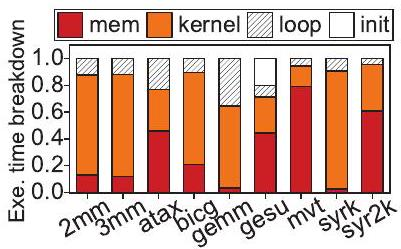
\includegraphics[max width=\textwidth]{2024_05_12_abeba8a85da5b5ec4c7bg-03(3)}
\end{center}

(a) Breakdown on CPU.

\begin{center}
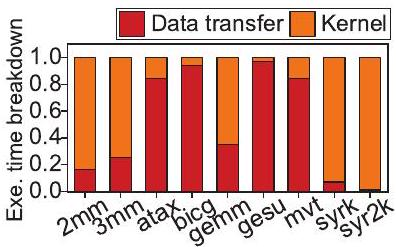
\includegraphics[max width=\textwidth]{2024_05_12_abeba8a85da5b5ec4c7bg-03(4)}
\end{center}

(b) Breakdown on GPU.\\
Fig. 3: Exe.time breakdown on CPU/GPU platforms.

\begin{center}
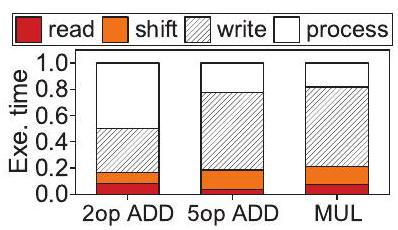
\includegraphics[max width=\textwidth]{2024_05_12_abeba8a85da5b5ec4c7bg-03(2)}
\end{center}

(a) Execution time breakdown.

\begin{center}
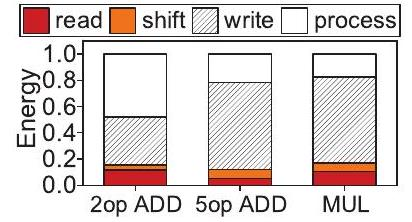
\includegraphics[max width=\textwidth]{2024_05_12_abeba8a85da5b5ec4c7bg-03}
\end{center}

(b) Energy cost breakdown.

Fig. 4: Execution time and energy cost breakdown of supported operations in CORUSCANT.

The statistics are collected from real platforms, which contain a 16-core processor [1] and a GPU [2], respectively. The memory access latency (cf. mem in Figure 3a) of small workloads (i.e., atax, bicg, gesu and mvt) accounts for $47.6 \%$ of the total execution time, on average, in the CPU-based computing system. This fraction increases up to $90.0 \%$ when executing the same workloads in the GPU-based computing system (cf. Data transfer in Figure 3b). This is because GPU devices require copying data between the main memory and its local memory, which increases the data migration overheads.

\section*{B. Process in Racetrack Memory}
To address the aforementioned challenges, prior works [45], [53], [77], [80] construct process-in-memory (PIM) from RM by placing customized computation units within or near the memory arrays. As data are directly processed within the memory, the PIM approaches avoid unnecessary data transfers between CPU/GPU and memory. However, the prior approaches still suffer from the overheads imposed by the data conversion between the memory cores and the PIM computation units.

To be specific, DW-NN [80] proposes to place CMOSbased arithmetic units near the RM arrays. The data are read from the RM arrays and then processed by the arithmetic units. The intermediate results are finally written back to the RM arrays for succeeding operations. Accommodating these intermediate results drastically increases the number of RM write operations, thereby exacerbating the electromagnetic conversion overheads between RM arrays and the arithmetic units. This is because RM suffers from long write latency and high write energy consumption. DW-AES [77] implements parts of AES encryption as RM shift operations thereby mitigating the data conversion overheads. However, this approach is highly algorithm-specific, which cannot be used to reduce such overheads in general matrix addition and multiplication.

The state-of-the-art work, CORUSCANT [53], leverages a unique characteristic of RM called Transverse Read [63] to mitigate the RM read overheads. To be precise, the transverse\\
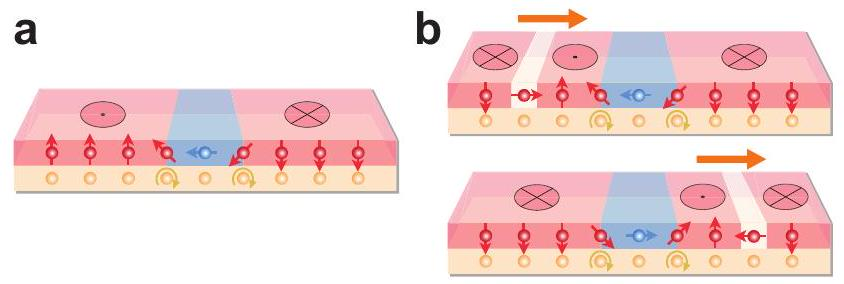
\includegraphics[max width=\textwidth, center]{2024_05_12_abeba8a85da5b5ec4c7bg-04(1)}

Fig. 5: Domain-wall nanowire logic mechanism.

read operation senses data out from a set of consecutive domains simultaneously rather than accessing each domain one by one. To reduce the operation delay further, CORUSCANT implements another mechanism called Transverse Write, which performs shift and write concurrently [73]. Although CORUSCANT provides lower latency and higher reliability than DW-NN owing to the new mechanisms, it still suffers from electromagnetic conversion overheads since it has to fetch/store intermediate results from/to RM arrays for each arithmetic computation. To figure out the impacts of data conversion overheads, we conduct an experiment by executing three common operations in CORUSCANT. Specifically, we adopt the statistics from the existing RM latency and energy models [26], [82] by considering the specific operation procedures employed in CORUSCANT to conduct the simulation. Figures $4 \mathrm{a}$ and $4 \mathrm{~b}$ show the execution time and energy consumption breakdown, respectively. The RM write operation accounts for $51.0 \%$ of the total execution time whereas only $30.1 \%$ of the execution time is used by the arithmetic units for computation. Similarly, the arithmetic units consume only $29.1 \%$ of the total energy (cf. Figure 4b). In contrast, the RM write operation becomes the major energy consumer. In summary, existing PIM solutions suffer from the overheads imposed by the data conversion between computation units and memory arrays. How to eliminate data conversion becomes the key to improving the performance and energy efficiency of PIM.

\section*{III. ARCHITECTURAL DESIGN}
\section*{A. Key Observation}
Recently, Luo et al. [46] discover a physical mechanism, which allows directly implementing Boolean logic operations on domain-wall nanowires. The authors also successfully fabricate a research sample to demonstrate the RM-based logic gates. Figure 5 depicts their approach. Specifically, by coupling magnetic metal and heavy metal, a domain-wall nanowire is integrated with domain-wall inverters. The inverters are used to enable a special interaction called Dzyaloshinskii-Moriya Interaction (DMI) [22]. The domains, domain-wall and domainwall inverter are shaded in red, white and blue in Figure 5, respectively. When the domains and domain-wall are driven by current (cf. the orange arrow in Figure 5b) and thus shift across the inverter, the domains will be logically inverted owing to DMI. Therefore, the inverter is equivalent to a NOT gate, as it inverts the logic values of the domains. Furthermore, two inputs, one bias, and one output domain can be coupled by DMI for more complicated logic operations. Figure 6 shows

\begin{center}
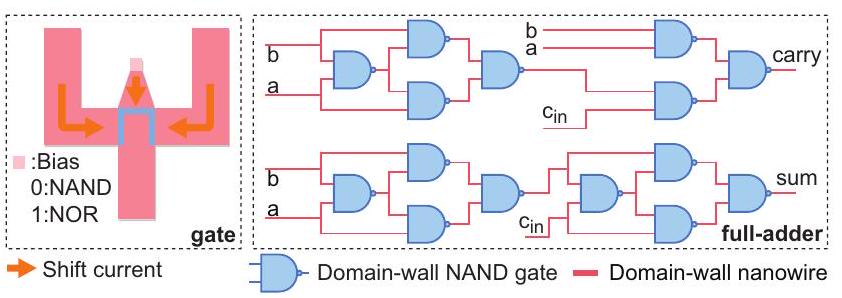
\includegraphics[max width=\textwidth]{2024_05_12_abeba8a85da5b5ec4c7bg-04}
\end{center}

Fig. 6: Domain-wall nanowire logic structures.

the structure of a domain-wall NAND/NOR gate. According to the given bias, the corresponding logic operation can be either NAND or NOR. Note that as all of the Boolean operations can be implemented by a combination of NOT, NAND and NOR operations, it is feasible to build a full-functional arithmetic unit based on domain-wall nanowires. We depict the one-bit full-adder built from domain-wall NAND gates in Figure 6.

\section*{B. StreamPIM Internal Architecture}
The aforementioned mechanism allows integrating arithmetic units tightly with memory arrays. Inspired by this key observation, we design processors and buses based on domain-wall nanowires and integrate them into the RM device, which significantly reduce the data conversion overheads within process-in-RM architecture.

Figure 7 shows the internal architecture of our design called StreamPIM. To serve regular memory accesses, we adopt the conventional RM architecture, which consists of three levels, including Bank, Subarray, and Mat. The bank is the top-level component and can be operated independently. All banks are connected by a shared internal bus, which supports the necessary inter-bank data transfers. A bank comprises of several subarrays and peripheral circuit modules, including global row buffers and row decoders. Each subarray can be accessed via local wordlines and bitlines to support memory access operations. In order to exploit the parallelism brought by multi-bank PIM architecture, we add a bank controller in each bank to serve the PIM operations internally. The bank controller manages its subarrays via PIM control lines. Furthermore, we adopt the local row buffer design inspired by a prior work [38], which is coupled with each subarray. This design improves the parallelism across different subarrays and allows a bank to accommodate more subarrays. Each subarray consists of several RM Mats, an RM Processor, and a set of internal RM Buses. While the RM mats are the basic memory arrays, the RM processor serves as the main computation unit to perform PIM function. The RM buses connect the mats and the processor for data transfers. These components are all built from domain-wall nanowires to minimize data conversion during processing.

\section*{C. RM Processor}
Our RM processor is designed for matrix computations including scalar addition, scalar multiplication, and vector dot product. To support scalar addition, we build an RM ripplecarry full-adder based on the 1-bit full-adder design depicted in Figure 6. The following describes how our RM processor design supports various multiplication operations.

\begin{center}
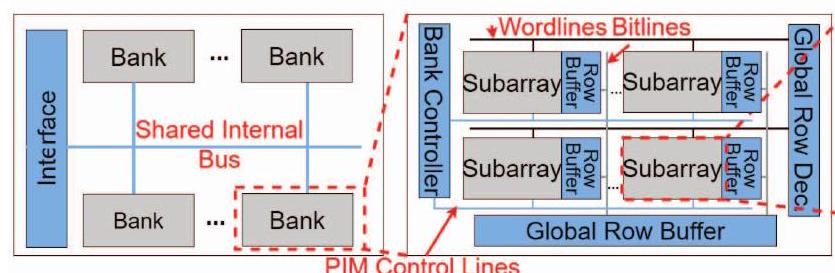
\includegraphics[max width=\textwidth]{2024_05_12_abeba8a85da5b5ec4c7bg-05(4)}
\end{center}

(a) Device

(b) Bank

\begin{center}
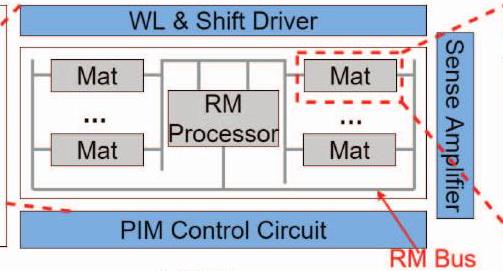
\includegraphics[max width=\textwidth]{2024_05_12_abeba8a85da5b5ec4c7bg-05(2)}
\end{center}

(c) Subarray

\begin{center}
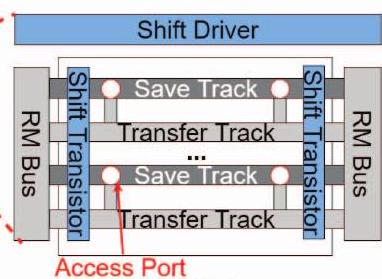
\includegraphics[max width=\textwidth]{2024_05_12_abeba8a85da5b5ec4c7bg-05(1)}
\end{center}

(d) Mat

Fig. 7: StreamPIM device architecture.

\begin{center}
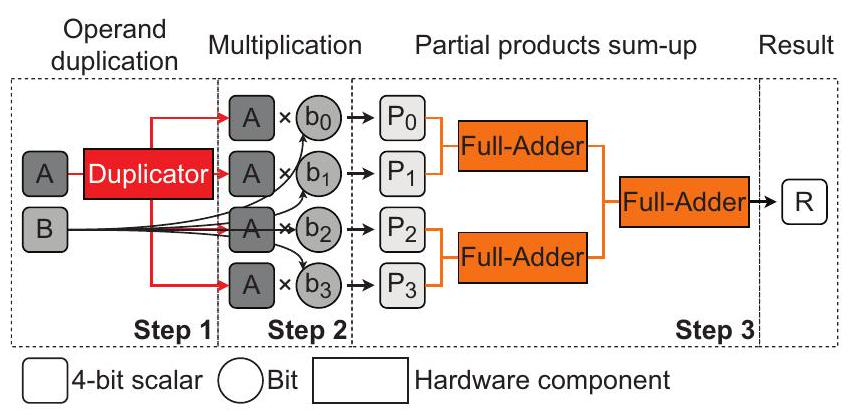
\includegraphics[max width=\textwidth]{2024_05_12_abeba8a85da5b5ec4c7bg-05(3)}
\end{center}

Fig. 8: 4-bit scalar multiplication example.

Scalar multiplication. Figure 8 shows the process for 4-bit scalar multiplication. Note that while our design supports 8 bit operands, we show only a 4-bit example owing to space limitations. Specifically, a hardware implementation of the scalar multiplication takes three steps: duplicating one of incoming operands (i.e., duplicating $A$ ), producing partial products (i.e., $A * b_{i}$ ), and summing up partial products.

The duplication step is non-trivial in RM as the shift operations only move data on domain-wall nanowires rather than duplicating data. Our solution is inspired by two materiallevel innovations in the RM domain called Fan-Out [46], [71] and Domain-Wall Diode [47]. Specifically, the fan-out approach designs a fan-out structure of domain-wall nanowire. By applying currents on both sides of the wires, the domain from the input is split into two domains when propagating through the fan-out point. On the other hand, similar to the traditional diode, a domain-wall diode allows the domains to propagate in only one direction when the diode is enabled. This mechanism makes it possible to flexibly control the data shift direction on nanowires. With these two mechanisms, we design a hardware component called Duplicator to perform data duplication. Figure 9 shows the structure of the duplicator and the four steps to duplicate data. To be precise, the duplicator is constructed from a customized domain-wall nanowire by following the fan-out mechanism. It places a domain-wall diode at one of the two branch nanowires. The duplication process is as follows. A shift operation propagates data toward two branch nanowires (step 1). The domain is duplicated when it reaches the branch nanowires according to the fan-out mechanism (step 2). A replica of the original data is transferred back to the original position once the domain-wall diode is enabled to avoid conflicts (step 3). Data returns to the original position and thus, is ready to be duplicated again (step 4). In the meantime, another replica is moved forwards to perform succeeding

\begin{center}
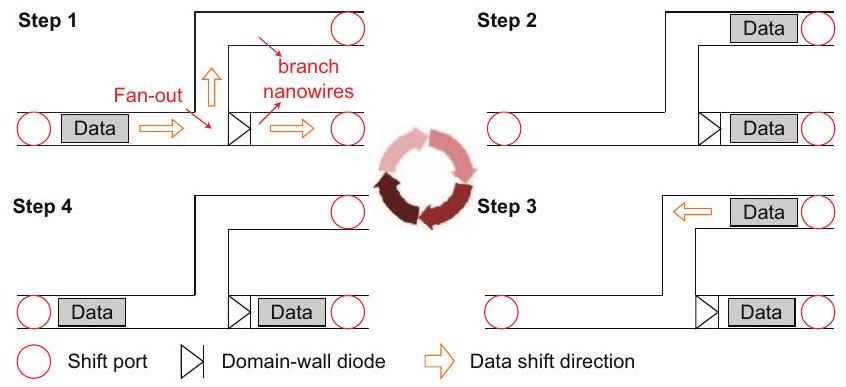
\includegraphics[max width=\textwidth]{2024_05_12_abeba8a85da5b5ec4c7bg-05}
\end{center}

Fig. 9: Duplicator structure and duplication steps.

operations. Note that an $n$-bit scalar multiplication needs to perform duplication by $n$ times, which costs an $n$-cycle stall. To tackle this challenge, we employ multiple duplicators in the processor to duplicate different parts of a vector simultaneously, thereby reducing the time consumption of duplication.

Partial products and their sum are calculated right after duplication (cf. steps 2 and 3 in Figure 8). Partial products can simply be generated by AND gates under binary data representation. To sum up partial products, we implement the multi-operand adder as an adder tree by leveraging the aforementioned RM full-adder (cf. Figure 6).

Vector dot product. The vector dot product operation is to sum up the results generated by the aforementioned scalar multiplication (cf. Result in Figure 8). To this end, we propose a design called Circle Adder, which consists of an $n$-bit full-adder, customized nanowires, and domain-wall diode. Figure 10 shows its structure and the four steps to add an incoming scalar multiplication product to the accumulated result. Specifically, the full-adder takes the incoming product value (d1) and the accumulated result (s1) as two operands to generate a new accumulated result (step 1). This result (s2) shifts across the domain-wall diode (step 2). s2 is then shifted back to the operand position via the circle-form nanowire, which is guided by the domain-wall diode (step 3). A new scalar product result ( $\mathrm{d} 2$ ) arrives at the operand position, preparing for the next iteration of addition (step 4). The addition process will be repeated until all of the scalar products are summed up. Then, the final result will be transferred out. Note that the circle adder can also execute scalar addition operations by simply shifting the operands across the full-adder without sending the result back. We multiplex the circle adder to execute both addition and dot product, which simplifies the hardware design. Pipelined processor. Figure 11 shows the overall structure of our RM processor that consists of the aforementioned duplicator, multiplier, adder tree, and circle adder. To improve

\begin{center}
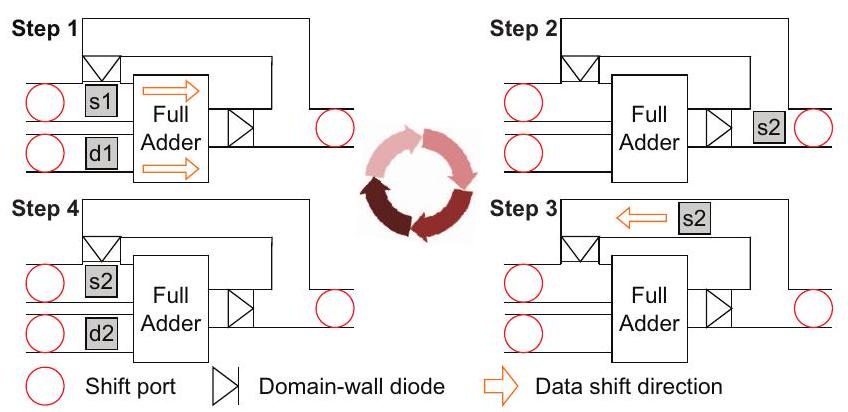
\includegraphics[max width=\textwidth]{2024_05_12_abeba8a85da5b5ec4c7bg-06(1)}
\end{center}

Fig. 10: Circle adder structure.

the processing throughput and hide the non-negligible latency of transferring data across domain-wall logic gates, we design the RM processor structure in a pipeline style. Specifically, we split the RM processor into four stages. When performing a vector dot product, a sequence of scalar operands is fetched into the RM processor. While one of the scalar operands is sent into the duplicator, the others are split into separated bits (Stage 1). The duplicator iteratively replicates the operand, which will be sent into the multiplier. The multiplier produces partial products from these replicas (Stage 2). An adder tree then sums up the partial products to generate the results of scalar multiplication (Stage 3). A circle adder collects all the results of scalar multiplications from the prior stage and adds them up (Stage 4). Note that our RM processor also supports other types of matrix operations. Specifically, a scalar multiplication bypasses circle-adder (Stage 4) since there is no need to add scalar multiplication results. A scalar addition bypasses the duplicator, multiplier and adder tree (Stages 1 to 3) while employing circle-adder as a simple adder. A vector addition can be performed by pipelining scalar additions. A scalarvector multiplication repeatedly duplicates its scalar operand and pipelines the following scalar-scalar multiplications.

\section*{D. RM Bus}
While both the RM array and the RM processor are built from domain-wall nanowires, transferring data between them requires electromagnetic data conversion owing to the traditional electrical bus. Inspired by the fact that the RM shift operation is a type of data transfer, we propose to build RM internal bus from domain-wall nanowires (RM bus).

Benefits. An RM bus brings two main benefits. First, transferring data via the domain-wall nanowires with shift operations can eliminate the read/write operations. Since a large-scale data-intensive application can generate a massive number of read/write operations, a well-designed RM bus will promisingly outperform a conventional electrical bus, which suffers from frequent electromagnetic conversion. Second, domain-wall nanowires allow multiplexing [8], which is infeasible in the traditional electrical bus. Specifically, a domain-wall nanowire consists of many domains, which can accommodate data from different RM arrays/processors. As a shift operation moves all the domains in a streaming fashion, different data can be transferred simultaneously without interference. In contrast, an electrical bus can only transfer a set of data at any given

\begin{center}
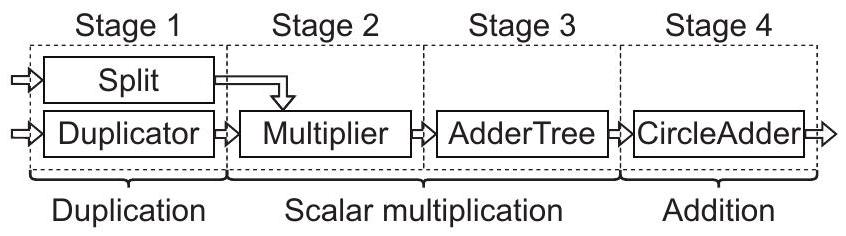
\includegraphics[max width=\textwidth]{2024_05_12_abeba8a85da5b5ec4c7bg-06}
\end{center}

Fig. 11: Pipelined RM processor.

\begin{center}
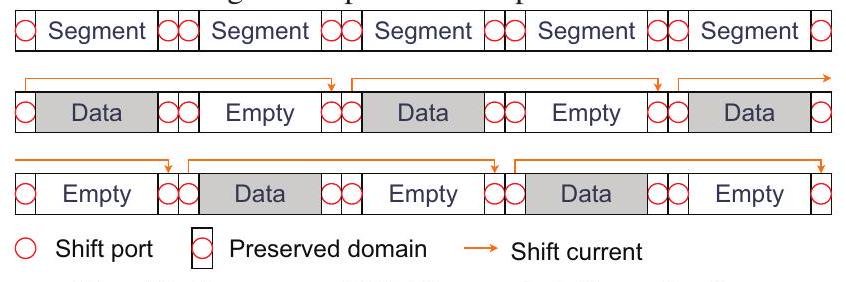
\includegraphics[max width=\textwidth]{2024_05_12_abeba8a85da5b5ec4c7bg-06(2)}
\end{center}

Fig. 12: Structure of RM bus and shift mechanism.

cycle. These benefits make domain-wall nanowires a potential contender for high-performance data transfers.

Challenges. During an RM shift operation, current pulses are applied to the domain-wall nanowire in a particular direction. Data then propagate through the domain-wall nanowire. However, this shift mechanism introduces three main challenges. First, the duration and density of current pulses need to be determined by the length of nanowires. However, it is hard to determine the length of nanowires for different transfers due to the various sources and destinations of the data. The uncertainty in duration and density of current makes it challenging to control the RM bus. Second, the data transfer latency of the RM bus is much higher than that of the electrical bus as domains can only propagate at a limited speed on nanowires [46]. Hence, transferring a single data costs multiple cycles, and the throughput can be severely limited if the data are transferred one by one. Third, when the length of nanowires increases, the over-shifting and under-shifting faults accumulate and become severe [63], which limits the transfer distance.

Our designs. Tackling the aforementioned challenges, we customize the structure of RM bus, which is shown in Figure 12. Specifically, StreamPIM groups a few consecutive domains in a domain-wall nanowire as a segment. Each domain-wall nanowire is then divided into multiple segments of the same length. On both sides of a segment, a domain is preserved for the shift port [26], which applies currents on the domainwall nanowire. When transferring data, a segment stays in one of two different conditions, either carrying data or empty. Figure 12 depicts these two conditions. The key insight of segment is to shift the data only by the length of a single segment in each cycle, confining the shift length. Hence, the non-determinism in duration and density of shift current can be avoided. However, to avoid data loss, the data segments should be shifted to empty segments during transfer. Thus, a set of data segments is always followed with empty segments in the transfer direction. Further, accidentally misaligned velocity between adjacent data segments also causes data loss. This feature requires a set of adjacent data segments to be shifted via a single shift current. As a result, there is still non-determinism in the duration and density of the shift current since the length of nanowires vary by the number of adjacent segments.

\begin{center}
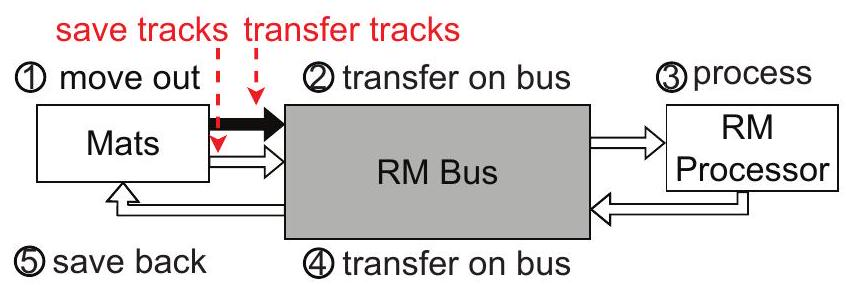
\includegraphics[max width=\textwidth]{2024_05_12_abeba8a85da5b5ec4c7bg-07}
\end{center}

Fig. 13: PIM data flow in a single subarray.

To completely remove this non-determinism, individual data segments are divided by empty segments. Consequently, a data segment is always followed by an empty segment in the direction of transfer (cf. Figure 12). Therefore, a single shift current is only applied to one data segment and the adjacent empty segment. Additionally, by simultaneously performing shift on all of such data-empty segment couples, data from different sources can be transferred concurrently in a pipelined fashion. This pipelined transfer drastically increases the data transfer throughput of RM bus compared to non-pipelined transfer, eliminating the impact of relatively long transfer latency. Furthermore, because the shift distance of each shift operation is restricted to only one segment, the shift fault issue can be mitigated. In summary, our design overcomes the aforementioned challenges by judiciously dividing the RM bus into segments, and can provide a significant performance improvement compared to traditional bus, as shown in our evaluation (cf. Figure 19).

\section*{E. Mat Design}
We propose a new mat design to eliminate electromagnetic conversions and realize non-destructive read operations, as shown in Figure 7d. A mat is essentially an array of domainwall nanowires. Note that the domain-wall nanowires in mats are particularly called racetracks. To communicate with the RM bus without electromagnetic conversion, racetracks in mats are extended and connected to the RM bus via domain-wall nanowires. Therefore, data can be moved between mats and RM bus by shift operations. However, data do not remain on the original mats after shift operations. Thus, shifting domains from mats to RM bus is a destructive-read operation. To perform a non-destructive read, data have to be copied onto rather than moved to RM bus. To this end, racetracks in a few mats are divided into two types: Save Track and Transfer Track. Save tracks are the basic units for accommodating data. They are connected with access ports to perform regular memory read/write operations. Transfer tracks are used for nondestructive reads and only send data to the RM bus. Rather than being connected to access ports, transfer tracks are connected to save tracks through fan-out domain-wall nanowires (cf. Figure 7d). By the fan-out mechanism, data can be copied onto transfer tracks without being erased from save tracks, and the replica can be transferred onto the RM bus. If a set of data needs to be read non-destructively, they will be transferred to the transfer tracks of the mats.

\begin{center}
\begin{tabular}{|c|c|}
\hline
Commands & Description \\
\hline
MUL src1,src2,des,size & Dot Product \\
\hline
SMUL src1,src2,des,size & Scalar-Vector Multiplication \\
\hline
ADD src1,src2,des,size & Vector Addition \\
\hline
TRAN src,des,size & Data Transfer \\
\hline
\end{tabular}
\end{center}

TABLE II: Vector processing commands (VPC).

\section*{F. Subarray Internal Data Flow}
Processing a PIM task inside a subarray involves mats, RM bus, and RM processor. The entire procedure is shown in Figure 13. Since data initially reside in mats, data first need to be transferred from mats to the RM processor. By applying shift operations, the data are moved from racetracks on mats to the RM bus (1). To perform non-destructive read, data are first moved from save tracks to transfer tracks and then from transfer tracks to RM bus. Then data are sent to the processor via the RM bus (2). The procedure will continue for several cycles. To eliminate this transfer overhead, the transfer procedure is designed in a pipelined fashion. A bunch of data will be fetched to the bus and transferred simultaneously. Once the data reach the RM processor, they are processed by different components including duplicator, multiplier, adder tree, and circle adder (3). Afterward, the data are transferred back to the destination mat via the RM bus (4), (5)).

Our design brings two main advantages to PIM tasks. First, magnetic signals stored in mats are never converted into electronic signals. The only operation imposed on data blocks is the shift operation, which has relatively low latency and energy costs compared to RM read/write operations. Second, since data are transferred on the RM bus and processed in the RM processor in a pipelined fashion, the throughput of PIM tasks can be significantly improved. These benefits are further elaborated on and examined in our evaluation part.

\section*{IV. Implementation and OptimIZATION}
\section*{A. Host-Device Interface}
To solve matrix computation tasks, the host needs to send commands to StreamPIM devices. The number of commands depends on the granularity of matrix computation interfaces exposed to the host. Basically, there are three possible granularity choices: scalar, vector, and matrix. The scalar granularity constrains a host PIM command to contain only two scalar values. The RM processor in turn produces a scalar result for each command. While scalar commands provide flexible programmability to the host, they generate significant communication overheads. In the worst case, up to $O\left(n^{3}\right)$ scalar operations can be transferred between the host and StreamPIM devices in a single matrix multiplication of size $n * n$. On the other hand, with matrix granularity, host PIM commands only need to indicate which input matrices are to be processed, thereby significantly reducing the communication overhead. However, this design offers the least programmability to the host and makes the execution much more complicated since PIM needs to deal with at least $\Omega\left(n^{2}\right)$ units of data in a single command. As a trade-off, we adopt vector granularity, for which a host PIM command indicates which vectors are

\begin{center}
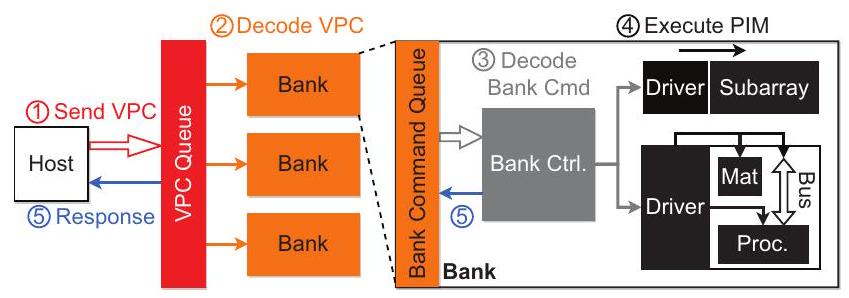
\includegraphics[max width=\textwidth]{2024_05_12_abeba8a85da5b5ec4c7bg-08(1)}
\end{center}

Fig. 14: Control flow of a PIM task.

to be operated. This design makes decoding procedure less complex, reduces the number of commands to $O\left(n^{2}\right)$ in a matrix multiplication and retains enough programmability for the host. Our customized PIM command is referred to as Vector Processing Command (VPC). Table II gives descriptions of different VPCs we use. The major types of matrix computation can be resolved by a combination of these VPCs, including addition, matrix-matrix multiplication, and matrix-scalar multiplication.

\section*{B. PIM Control Flow}
Figure 14 depicts the control flow of a PIM computation task. There are five steps from host commands to hardware execution. First, the host sends PIM VPCs to the StreamPIM device (1). The commands are decoded and distributed to related banks and subarrays, and then executed by the RM bus and processor (2), (3) and (4). After the execution completes, a response message is sent back to the host (5).

VPC sending and responding. During the execution of a PIM task, the host continually sends VPCs to StreamPIM devices. To fully exploit the parallelism of the multi-bank architecture, commands are sent in an asynchronous send-response style, which has been explored in prior research on DRAM and NVM systems [49], [61]. The incoming commands from the host are buffered in a VPC queue within StreamPIM devices. After a VPC completes execution, a response message will be sent back to the host. This asynchronous design allows the device to execute VPCs on different banks simultaneously, which efficiently exploits the multi-bank architecture.

VPC decoding and distributing. After receiving a VPC, a StreamPIM device decodes it into one or multiple bank commands as shown in Figure 14. Specifically, a VPC is executed inside a single subarray to avoid unnecessary data movement of intermediate results among subarrays. Therefore, if both the vector operand and result are in the address range of a single bank, the VPC is sent directly to the target bank. Otherwise, several read/write commands are sent to the corresponding banks for data preparation. These commands collect vector operands and send them to the processor in a particular bank. Afterward, the results are saved to the destination bank via read/write commands.

To execute bank commands on a subarray, the bank controller decodes commands into operations and manages the driver to execute them on the RM bus and RM processor. For example, a vector dot product command is decoded to (1) two data transfer operations that fetch vector operands from RM mats to RM processor; (2) a group of scalar multiplication operations; (3)

\begin{center}
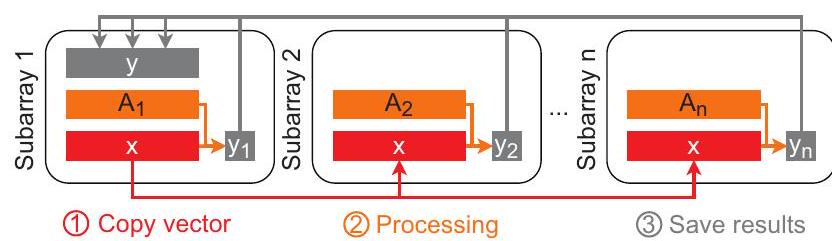
\includegraphics[max width=\textwidth]{2024_05_12_abeba8a85da5b5ec4c7bg-08}
\end{center}

Fig. 15: Example of distribute execution.

a group of scalar addition operations that sum up the results of scalar multiplication to generate the final result; (4) a data transfer operation that stores the result to the destination mat. Similar to VPC decoding, if the operands locate at different subarrays, several read/write operations are generated to fetch operands and store results.

\section*{C. Parallelism Optimization}
Subarray-level parallelism. Since a VPC is executed by a single RM processor, performance is limited by the device clock frequency. To mitigate the impact, we propose a customized data placement method for matrix computation. Take the execution of $y=A x$ as an example, where $x, y$ are $n$-dimensional vectors and $A$ is an $n * n$ matrix. The entire task is resolved into $n$ VPCs as dot products between $x$ and different rows in $A$, denoted as $y_{1}=A_{1} x, y_{2}=A_{2} x, \ldots, y_{n}=A_{n} x$. A naive base method is to place different rows in sequential addresses. Thus, a single subarray is responsible for the execution of multiple $y_{i}=A_{i} x$ VPCs. Since a subarray only contains a single processor, these VPCs will be executed serially, which harms parallelism and degrades performance. To address this problem, we propose a distribute method as shown in Figure 15. The different rows of $A$ are stored in different subarrays. Before data processing, StreamPIM performs additional data preparation by copying $x$ into different subarrays (1) via inter-subarray and inter-bank communication. Then, different $y_{i}=A_{i} x$ VPCs can be executed simultaneously on these subarrays (2)). The results produced by different subarrays are then collected and transferred to the destination subarray containing $y$ (3). In case of matrix multiplication (e.g., $A * B$ ), the distribute optimization divides the computation into multiple matrix-vector multiplications (e.g., $A * B_{i}$, where $B_{i}$ are the columns of $B$ ). It then performs the computations of $A * B_{i}$ with the aforementioned optimization. During the execution of $A * B_{i}$, the distribute copies $B_{i}$ on demand to different subarrays where the rows of $A$ reside, conducts vector dot products, and collects the results.

The distribute optimization constrains the vector length in a VPC so that a vector can be entirely placed in a single subarray. In most cases, this is achievable because the subarray proposed in our design has a large memory capacity (only $1 / 2048$ of the total memory capacity in our experiments). To handle an oversized vector which is larger than a subarray's capacity, StreamPIM employs a slicing strategy [14], [65] to distribute different parts of the vector to different subarrays, process them and then collect the results.

Mitigating operation blocking. Performing distribute optimization needs necessary inter-subarray and inter-bank data copying to distribute the vectors to different subarrays. This

\begin{verbatim}
task = create_pim_task() // Step 1
// A, B, C are pre-allocated arrays
task.add matrix(A, size1, size2) // Step 2
task.add_matrix(B, size2, size3)
task.add matrix(C, size1, size3)
task.add-operation(MUL, A, B, C)
task.run()
// Step 3
\end{verbatim}

Fig. 16: Example of programming interfaces.

copying is mainly conducted by read/write operations, while the in-subarray transfer and computation are performed via RM shift operations. However, for the sake of data integrity, the shift operations cannot be executed simultaneously with read/write operations in a single subarray. Therefore, when a subarray is executing computations, read/write operations targeting this subarray will be blocked. Furthermore, the computations on other subarrays that need data from these read/write operations will also be blocked. Consequently, computations on different subarrays are serialized, harming the parallelism and degrading overall performance.

To resolve this issue, we propose a method called unblock. First, in a single matrix computation task, the operands and results are placed in different predefined subarray sets that do not overlap. With this layout optimization, the read/write and computation operations of one matrix computation task are decoupled into different subarray sets, mitigating blocking between these operations. Second, the execution order of computation and read/write operations is rearranged so that they are interleaved to access different subarrays. By doing so, the computation and read/write operations do not block each other on the same subarray. This also mitigates operation blocking among bank commands. With distribute and unblock optimizations, the subarray-level parallelism can be fully exploited, improving the overall performance.

\section*{D. Programming Interface}
To bridge the gap between matrix-grained tasks and vectorgrained commands, we propose a set of programming interfaces and deliver them as a runtime library.

In general, it takes three steps to program a StreamPIM task. Figure 16 shows an example. In Step 1, a PIM task is created. Conceptually, a task deals with a set of matrix operands (sources and destinations) and computation operations. These operands and operations are expected to be interdependent, making it beneficial to optimize them as an integral process. Programmers can inform the task of the exact operands and operations via interfaces (Step 2). The task then decides the specific optimization strategy by using the optimizations described in Section IV-C. In the example shown in Figure 16, when matrices are added (line 3-5), through the layout optimization proposed in distribute and unblock, the task determines the subarrays that the vectors of these matrices need to be distributed to during computation. This layout optimization uses TRAN VPCs (cf. Table II) to perform necessary copying. When operations are added (line 6), the task decides the VPCs needed for computing, and rearranges the order of all VPCs through the unblock method. Since the optimization strategy keeps

\begin{center}
\begin{tabular}{|c|c|}
\hline
Processor & 16 cores, X86 ISA, 3.7 GHz, out-of-order \\
\hline
Cache & $512 \mathrm{KiB}$ L1-cache, 8 MiB L2-cache \\
\hline
DW memory & \begin{tabular}{c}
$8 \mathrm{GiB} ; 2400 \mathrm{MHz}$ IO bus speed \\
bank-subarray-mat: $32-64-16 ; 256 \mathrm{KiB} / \mathrm{mat}$ \\
\end{tabular} \\
\hline
core frequency: $100 \mathrm{MHz}$ &  \\
StreamPIM & \begin{tabular}{c}
copos \\
in-processor duplicator count: 2 \\
save track/transfer track: $512 / 512$ (per mat) \\
latency: read: 3.91 write: 10.27 shift: 2.13 (ns) \\
energy: read: 3.80 write: 11.79 shift: 3.26 (pJ) \\
PIM energy: add: 0.03 mul: 0.18 (pJ) \\
fabrication process: $32 \mathrm{~nm}$ \\
\end{tabular} \\
\hline
\end{tabular}
\end{center}

TABLE III: CPU and memory configurations.

\begin{center}
\begin{tabular}{|cccc|}
\hline
Benchmark & Process task & \#PIM-VPC & \#move-VPC \\
\hline
$2 \mathrm{~mm}$ & $E=\alpha A B C+\beta D$ & $7.37 \times 10^{6}$ & $7.36 \times 10^{6}$ \\
$3 \mathrm{~mm}$ & $G=(A B)(C D)$ & $1.19 \times 10^{7}$ & $1.18 \times 10^{7}$ \\
gemm & $C^{\prime}=\alpha A B+\beta C$ & $4.61 \times 10^{6}$ & $4.60 \times 10^{6}$ \\
syrk & $C^{\prime}=\alpha A A^{T}+\beta C$ & $6.77 \times 10^{6}$ & $6.76 \times 10^{6}$ \\
syr2k & $C^{\prime}=\alpha A B^{T}+\alpha B A^{T}+\beta C$ & $1.36 \times 10^{7}$ & $1.35 \times 10^{7}$ \\
atax & $y=A^{T} A x$ & $4.00 \times 0^{3}$ & $8.40 \times 10^{3}$ \\
bicg & $q=A p, s=A^{T} r$ & $3.60 \times 10^{3}$ & $8.00 \times 10^{3}$ \\
gesu & $y=\alpha A x+\beta B x$ & $5.60 \times 10^{3}$ & $8.40 \times 10^{3}$ \\
mvt & $x_{1}=x_{1}+A y_{1}, x_{2}=x_{2}+A^{T} y_{2}$ & $8.00 \times 10^{3}$ & $1.60 \times 10^{4}$ \\
\hline
\end{tabular}
\end{center}

TABLE IV: Workload characteristics.

adjusting as operands and operations are continually added during step 2, the actual computation will not be performed until the call of task. run (), which denotes a stabilized task. Based on the optimization strategy, the task conducts layout optimizations and generates VPCs in the optimized order to perform the computation (Step 3).

\section*{V. Evaluation}
\section*{A. Experimental Setup}
Methodology. To explore the full design space of the RMenabled systems, we replace the existing main memory system in a full system simulator, i.e., gem5 [10], [20], with the RM latency model. The latency model is derived from popular NVM memory modeling tools (RTSim [34] and NVSim [18]). To precisely simulate the PIM latency in RM, we build a cycleaccurate simulator from scratch. Our simulator adopts the model of domain-wall logic structures, which is derived from the real research samples in the laboratory environment [46]. Table III lists the detailed configurations of the CPU platform and the domain-wall memory in our experiments. Specifically, we adopt a 16-core X86 processor [1] and an 8GB domain-wall memory [26]. The domain-wall memory is organized as 32 banks, including 8 PIM banks and 24 memory banks. Each PIM bank integrates RM processors in subarrays to perform matrix computation while the memory banks only serve the memory requests. We set the memory core frequency to $100 \mathrm{MHz}$ based on the existing studies [18], [46], which guarantees the functionality of all the pipeline components in our design. We adopt the energy configurations of RM from prior works [26], [82] and derive the energy statistics of our RM processor by referring to the real research samples [46].

Computing platforms. We set up 6 different computing platforms for evaluation: (1) CPU-RM: the traditional computing platform that employs CPU and RM; (2) CPU-DRAM: the traditional computing platform that employs CPU and

\begin{center}
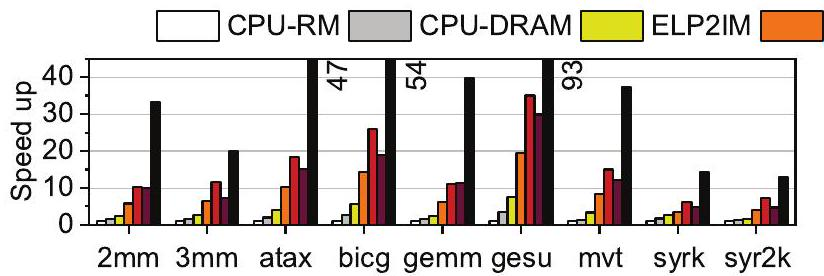
\includegraphics[max width=\textwidth]{2024_05_12_abeba8a85da5b5ec4c7bg-10(1)}
\end{center}

Fig. 17: Performance speed up compared to CPU-RM.

\begin{center}
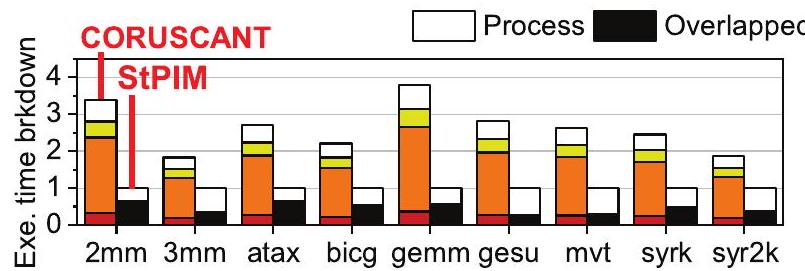
\includegraphics[max width=\textwidth]{2024_05_12_abeba8a85da5b5ec4c7bg-10(3)}
\end{center}

Fig. 19: Exe. time breakdown normalized to StPIM.

DDR4 DRAM with $2400 \mathrm{MHz}$ IO speed; (3) StPIM: the StreamPIM (abbreviated as StPIM) platform with 512 PIMsubarrays and the optimizations proposed in Section IV(i.e., distribute and unblock); (4) StPIM-e: similar to StPIM, but the in-subarray RM buses are replaced with traditional electrical buses, which helps us to analyze the efficiency of RM bus; (5) ELP2IM: implementation of a state-of-the-art process-in-DRAM work [78], which performs arithmetic operations via serialized bit-level logical operations; (6) FELIX: implementation of a state-of-the-art process-inNVM work [19], performing arithmetic operations via serialized bit-level logical operations; (7) CORUSCANT: implementation of a state-of-the-art process-in-RM work [53]. Note that we set the same configurations in ELP2IM, FELIX, CORUSCANT, and StreamPIM, including the memory core frequency and fabrication process of domain-wall nanowires (cf. Table III). We also ignore the inter-subarray and bank data movements in ELP2IM, FELIX and CORUSCANT to make them ideal cases. All the platforms omit the cost of error resilience support for fairness.

Workloads. To quantitatively evaluate our designs on matrix computation, we select 9 representative workloads from polybench [59], covering a wide range of linear-algebra applications [9], [83]. The details of evaluated workloads are listed in Table IV. Note that gesu is the abbreviation of gesummv in Table IV and the following figures. These workloads consist of different matrix processing operations, including addition and multiplication of matrices, vectors, and scalars. To better illustrate the capabilities of our design on large datasets, we set the vector dimension to 2000, which is a common configuration in polybench. For architectural simulation, we generate VPC traces for each workload by modifying the source codes of polybench and fitting them into the optimizations proposed in Section IV-C with the programming interfaces discussed in Section IV-D. Our cycleaccurate simulator then extracts all VPC-related information from these traces and processes them. Columns \#PIM-VPC and \#move-VPC in Table IV represent the VPC counts of processing and data movement in each trace, respectively.

\begin{center}
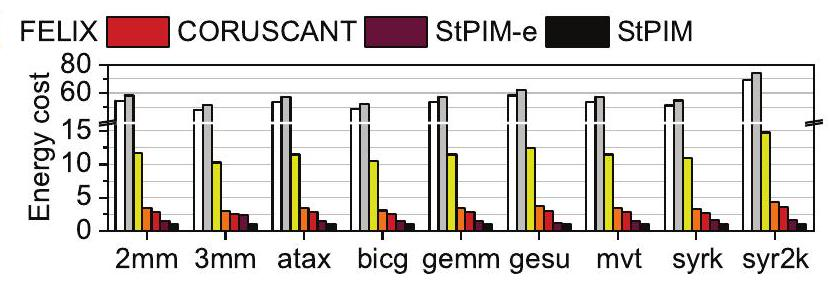
\includegraphics[max width=\textwidth]{2024_05_12_abeba8a85da5b5ec4c7bg-10}
\end{center}

Fig. 18: Energy cost normalized to StPIM.

\begin{center}
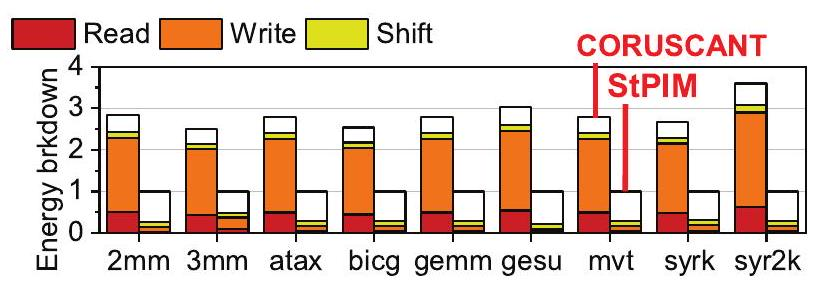
\includegraphics[max width=\textwidth]{2024_05_12_abeba8a85da5b5ec4c7bg-10(2)}
\end{center}

Fig. 20: Energy cost breakdown normalized to StPIM.

\section*{B. Overall Performance}
Figure 17 shows the performance of different computing platforms for various workloads in terms of the speed up compared to CPU-RM. We provide the performance of CPU-DRAM to better illustrate the absolute performance of RM-based architecture. Specifically, CPU-DRAM outperforms CPU-RM by $1.5 \times$, on average, due to the benefits of shorter access latency and higher bandwidth. StPIM-e achieves $12.7 \times$ average speed-up compared to CPU-RM by efficiently eliminating the data transfer overheads with PIM technique. Additionally, the distribute and unblock optimizations help to fully exploit the subarray-level parallelism, resulting in significant performance gain. StPIM successfully reduces the data transfer overheads between RM mats and processors by leveraging the internal RM bus. These overheads are further hidden with pipelined transferring of RM bus. Thus, StPIM achieves $3.1 \times$ and $39.1 \times$ average performance compared to StPIM-e and CPU-RM, respectively. On the other hand, although the ideal CORUSCANT solution has $15.6 \times$ performance compared to CPU-RM baseline, StPIM still outperforms CORUSCANT by $2.5 \times$, on average. This is because StPIM can amortize the execution overheads of scalar operations with the pipeline architecture, whereas CORUSCANT suffers from heavy data conversion overheads, leading to longer execution time. Because ELP2 IM only supports bit-level logic operations, its performances of arithmetic operations are limited by the serialized bit-level logical operations, which restrict its internal parallelism. As a result, ELP2IM only achieves a $3.6 \times$ speed-up compared to CPU-RM baseline. FELIX, by executing computation on NVM, removes the precharge phases required by DRAM, and improves its performance to $8.7 \times$ of CPU-RM. However, the performance of FELIX is still limited by serialized bit-level operations. In contrast, CPRUSCANT and StPIM outperform FELIX by $1.8 \times$ and $4.5 \times$, and outperform ELP2IM by $4.4 \times$ and $10.9 \times$, respectively.

Figure 19 shows the execution time breakdown of CORUSCANT and StPIM, which are normalized to StPIM. The execution time is split into the exclusive data transfer time

\begin{center}
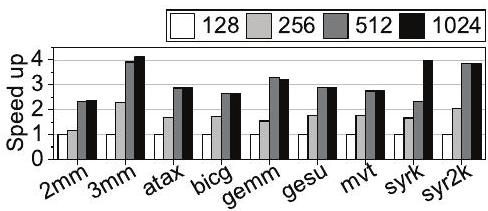
\includegraphics[max width=\textwidth]{2024_05_12_abeba8a85da5b5ec4c7bg-11}
\end{center}

Fig. 21: Performance of different PIM subarray counts.

\begin{center}
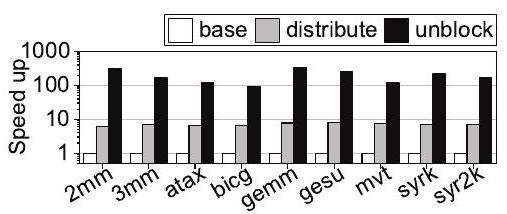
\includegraphics[max width=\textwidth]{2024_05_12_abeba8a85da5b5ec4c7bg-11(1)}
\end{center}

Fig. 22: Performance of different optimizations. (including Read, Write and Shift), the exclusive processing time (Process) and the overlapped parts (Overlapped). For CORUSCANT, Read, Write and Shift represent for the execution time of RM read, write and shift operations, respectively. For StPIM, Shift represents for in-subarray data transfer overheads, while Write together with Read represents for inter-subarray and inter-bank data movement overheads. The results show that CORUSCANT suffers from heavy data transfer overheads $(81.82 \%$ on average). In contrast, by performing data transferring and processing in a pipelined fashion, StPIM hides the transfer time by processing time, reducing the exclusive data transfer overheads to below $1.0 \%$.

\section*{C. Energy Consumption}
Figure 18 shows the average energy consumption of different platforms, which are normalized to StPIM. As the memory devices (i.e., DRAM and RM) require relatively less energy than computation units and data transfer processes, the energy consumption of DRAM-based architectures (CPU-DRAM) is close to RM-based architectures (CPU-RM). By eliminating the energy-intensive process of transferring data between memory and computation units, StPIM achieves $58.4 \times$ energy efficiency compared to CPU-DRAM baseline. Compared to FELIX and CORUSCANT, StPIM $3.5 \times$ and $2.8 \times$ higher energy efficiency, respectively. This is because StPIM mainly performs data transferring and processing via energy-efficient shift operations, while FELIX and CORUSCANT rely on electromagnetic conversion operations (i.e., read and write), which consume more energy. Compared to ELP2IM, StPIM achieves $11.7 \times$ energy efficiency, because it removes the energy-thirsty refresh and precharge operations required by DRAM technology. Further, because the RM processor consumes less energy than CMOS-based units, StPIM-e achieves $2.2 \times$ and $1.8 \times$ improvements over FELIX and CORUSCANT, respectively. However, because the electrical bus is less energyefficient than the RM bus, StPIM-e consumes an average of $1.6 \times$ more energy than StPIM.

Figure 20 presents the energy cost breakdown of CORUSCANT and StPIM, normalized to StPIM. Since StPIM transfers data via shift operations instead of electromagnetic conversion, the average energy fraction of data transfer in StPIM is reduced to only $30 \%$. In contrast, CORUSCANT incurs an $86 \%$ average energy overhead due to inefficient electromagnetic conversion operations.

\section*{D. Sensitivity Testing}
PIM subarray count. We evaluate the impacts of PIM subarray count on the performance of StPIM by adjusting the number

\begin{center}
\begin{tabular}{|c|c|c|c|c|}
\hline
Segment size & 64 & 256 & 512 & 1024 \\
\hline
Execution time & $+2.33 \%$ & $+0.58 \%$ & $+0.29 \%$ & $0 \%$ \\
\hline
Energy cost & $-0.1 \%$ & $-0.05 \%$ & $-0.04 \%$ & $0 \%$ \\
\hline
\end{tabular}
\end{center}

TABLE V: Average performance and energy comparison between different bus segment sizes (normalized to 1024).

of subarrays per bank and the memory capacity per subarray. Figure 21 shows the performance result, which is normalized to the 128 -subarray baseline (128). Compared to baseline, employing 256, 512 and 1024 subarrays can improve average performance by $1.74 \times, 3.0 \times$, and $3.2 \times$, respectively. With more subarrays, the average performance is expected to get saturated since the data dependency limits higher parallelism. Optimization. We evaluate the benefits of distribute and unblock optimizations by selectively applying them in the test. Figure 22 shows the results normalized to base (i.e., no optimization). The performance of base is limited by the low memory core frequency and under-utilization of RM internal parallelism. Employing distribute yields a $7.1 \times$ average performance compared to base. This is because distribute can better exploit the subarray-level parallelism by distributing computation among different subarrays. However, the performance of distribute is still limited by the operation blocking. By successfully overcoming this problem, unblock achieves $199.7 \times$ higher average performance compared to base.

Segment size. As RM buses transfer data in segments, the segment size affects transfer performance. Since data can only be transferred by one segment in a cycle, shrinking segment size increases the segment count on RM buses, requiring more cycles to transfer data between RM arrays and processors. However, because in most of the cycles, bus transfer is performed simultaneously with computation and its overheads are hidden (cf.Section V-B), such impact is minimal. Table V gives a sensitivity testing results. Shrinking segment size from 1024 to 64 only incurs $2.33 \%$ average overheads on overall performance. On the other hand, increasing segment size requires more energy due to larger shift current. However, this energy overhead is compensated by reducing the number of shift operations, thanks to decreased segment count. Consequently, the energy cost remains nearly unchanged as shown in Table V. In our evaluation, we choose 1024 as the default setting to demonstrate the best performance of our design.

\section*{E. End-to-end Performance}
To demonstrate the end-to-end performance, we adapted two DNN applications to StreamPIM, including MLP (multilayer perceptron) [41] and BERT [16]. Since these DNN\\
applications include various types of computation operations, we only offload the matrix multiplication and addition to StreamPIM while relying on CPU to process the unsupported operations (i.e., nonlinear operations). Figure 23 depicts the execution speed-up of diverse computing platforms against CPU-DRAM. Because the nonlinear layers in MLP are a small portion of MLP inference, StreamPIM achieves a $54.77 \times$ speed-up compared to CPU-DRAM by significantly accelerating the matrix computation. In addition, StreamPIM improves the performance by $1.86 \times$ compared to CORUSCANT, owing to its specific optimizations for matrix operations. On the other hand, since BERT involves with more nonlinear operations (e.g., matrix normalization), StreamPIM shows relatively less performance gain. Nevertheless, by accelerating the critical matrix-computation part in BERT inference, StreamPIM still achieves a $4.49 \times$ and $1.97 \times$ better performance, compared to CPU-DRAM and CORUSCANT, respectively.

\section*{F. Fabrication Process}
Since all the arithmetic operations in StreamPIM are performed via shift operations, the energy cost are dominated by the shift current level and fabrication process, and are calculated via a formula and statistics derived from the research [46]. When the domain scale shrinks down, the energy cost per gate decreases drastically. For example, the energy cost per gate will drop from $20 \mathrm{pJ}$ to $0.0008 \mathrm{pJ}$ when the domain scale shrinks from $1.0 \mu \mathrm{m}$ to $32 \mathrm{~nm}$ scale. In our evaluation, we leverage CORUSCANT-compatible configuration (i.e., $32 \mathrm{~nm}$ ), under which the energy consumption of ADD and MUL operation can be $0.03 \mathrm{pJ}$ and $0.18 \mathrm{pJ}$, showing an outstanding energy efficiency compared with CMOS-based arithmetic units.

\section*{G. Area Overheads}
We analyse the area breakdown of our design by estimating the number of domains in different components. The configurations of the mat number per subarray, the total PIM subarray and the total subarray number are trade-off between performance and area overhead. In our default configurations, we assume each subarray contains 16 RM mats, in which 2 mats have transfer tracks. In addition, we assume 512 PIM subarrays and 2048 subarrays in total. The RM bus and RM processor only occupy $1.8 \%$ and $0.1 \%$ of the total area in a RM device, respectively. On the other hand, the area overhead of transfer tracks is only $3.1 \%$ while that of the added control logic is only around $1.0 \%$, compared to the bank area according to a prior research [82]. The results show that our design strikes a good balance between the performance and area consumption.

\section*{VI. RELATED WORKS AND DISCUSSION}
PIM in PCRAM and STT-MRAM. Multiple prior works have proposed PIM architectures based on PCRAM and STTMRAM. For example, a typical process-in-PCRAM architecture, Pinatubo [43], simultaneously opens two memory rows and senses them via adjusted threshold voltages to perform bitwise logic operations. Another work [31] proposes a similar method in STT-MRAM. Other research [6], [19], [21] propose in-cell Boolean operations to avoid adding complex sensing circuits. These approaches can only support bitwise logic operations (e.g., AND and OR). Thus, an arithmetic operation takes multiple steps, creating massive intermediate results and generating intensive memory reads and writes. In contrast, as StreamPIM employs customized arithmetic units to support advanced arithmetic operations such as addition, multiplication and dot product, it significantly reduces the amount of intermediate results during the matrix computation. PIM in crossbar ReRAM. Crossbar designs [14], [65], [70], as typical implementations of process-in-ReRAM architecture, are capable of performing vector dot product. In a crossbar architecture, the data in a column of cells and the input voltages on bitlines are regarded as two vector operands. The current on the wordline will then form the dot product of these two vectors. Furthermore, with MLC (multi-level cell) technique, a cell can store more than one bit, and the input voltages can also be adjusted to multiple levels. Thus, crossbar dot product can obtain higher precision. Crossbar-based PIM architectures can achieve high throughput and energy efficiency. However, the essential analog-digital-conversion (ADC) for MLC approaches [14] incurs non-negligible overheads. Meanwhile, SLC (single-level cell) designs [70] can only support basic bit-level operations, requiring multiple steps and massive intermediate results to perform high-level computations. In contrast, StreamPIM can eliminate ADC overheads by storing and processing data in digital form, and support advanced arithmetic operations to reduce the amount of intermediate steps and results.

Hardware implementation. As a newly proposed technology, there are still multiple steps to bring domain-wall based processor into massive production. One concern is the reliability of processor. In the proof-of-concept experiment, several cascaded circuits demonstrate promising reliability [46]. Several works have also been proposed to improve reliability of DMI [44], [75]. Another concern falls on RM bus, which is mainly affected by shift faults. Multiple works have successfully mitigated or even avoided the shift fault issue [35], [54]. StreamPIM can leverage these methods to improve its hardware reliability from physical/material perspective. Furthermore, StreamPIM can also adopt architectural supports from [53] (i.e., redundancy design) to compensate for error tolerance.

Supported operations. In this paper, StreamPIM focuses on accelerating the most fundamental operations in dataintensive and compute-intensive applications (i.e., addition and multiplication). To support these operations, StreamPIM constructs customized adder and multiplier from scratch based on logic gates. By implementing and integrating other specified processors (e.g., divider, square-root extractor and floating-point processor [5], [29], [32], [52], [76], [81]), StreamPIM can be extended to support plenty of more arithmetic operations and data representation types. These extensions can make StreamPIM suitable for a wider range of computation kernels (e.g., FFT and DNN training). Since the main purpose of this work is architectural design and optimization for processin-RM device, the implementation details of aforementioned extensions, which require dedicated designs and optimizations,\\
are omitted due to space limits and left for future works.

Programming interface and device control. In the evaluated applications, the source codes define matrix-grained tasks while our StreamPIM device executes scalar-grained computations. To bridge the gap between application source codes and computation on RM devices, StreamPIM proposes a vectorgrained interface level sitting between these two levels, which is discussed in IV. Being aware of previous works in both academic and industrial domains [4], [14], [66], StreamPIM chooses to deliver this interface level as a suite of libraries, including code compiler and device driver. This design gives the interface level the ability to (1) extract the computation graph from applications and decide the optimization strategy, including data placement optimization and command reordering, plus (2) translate the computation and optimization into a device-level (i.e., physical) representation and conduct them.

\section*{VII. ConClusion}
We propose StreamPIM, a new processing-in-RM design, which improves performance and energy efficiency for matrix computation tasks substantially. StreamPIM directly constructs a matrix processor from the domain-wall nanowires, thereby enabling RM to serve both computation and I/O tasks. It also integrates a domain-wall nanowire based bus to eliminate the conversion overheads. Our evaluation results show that StreamPIM achieves performance speedup and energy saving compared to the state-of-the-art process-in-RM solutions.

\section*{ACKNOWLEDGEMENT}
We thank anonymous reviewers for their constructive feedback. We thank all the joys brought by Ran. This work is mainly supported by the National Key Research and Development Program of China under Grant No. 2023YFB4502702, the Natural Science Foundation of China under Grant No. 62332021, and the Fundamental Research Funds for the Central Universities, Peking University. Dr. Li is supported in part by the National Natural Science Foundation of China under Grant No. 62202396 . Dr. Luo is supported in part by the National Key Research and Development Program of China under Grant No. 2022YFA1203904 and the National Natural Science Foundation of China under Grant No. 52271160. Dr. Sun is supported in part by the National Natural Science Foundation of China under Grant No. 62032001. The corresponding author is Jie Zhang.

\section*{REFERENCES}
[1] "Amd ryzen"TM 9 5950x desktop processors," \href{https://www.amd.com/en/}{https://www.amd.com/en/} products/cpu/amd-ryzen-9-5950x, 2020.

[2] "Geforce rtx 3080 family," \href{https://www.nvidia.com/en-us/geforce/}{https://www.nvidia.com/en-us/geforce/} graphics-cards/30-series/rtx-3080-3080ti/, 2021.

[3] M. Abadi, P. Barham, J. Chen, Z. Chen, A. Davis, J. Dean, M. Devin, S. Ghemawat, G. Irving, M. Isard, M. Kudlur, J. Levenberg, R. Monga, S. Moore, D. G. Murray, B. Steiner, P. A. Tucker, V. Vasudevan, P. Warden, M. Wicke, Y. Yu, and X. Zhang, "Tensorflow: A system for large-scale machine learning," ArXiv, vol. abs/1605.08695, 2016.\\
[4] N. Agarwal, D. W. Nellans, M. W. Stephenson, M. O'Connor, and S. W. Keckler, "Page placement strategies for gpus within heterogeneous memory systems," Proceedings of the Twentieth International Conference on Architectural Support for Programming Languages and Operating Systems, 2015. [Online]. Available: \href{https://api.semanticscholar.org/CorpusID:207221462}{https://api.semanticscholar.org/CorpusID:207221462}

[5] M. Anas, R. S. Padiyar, and A. S. Boban, "Implementation of cordic algorithm and design of high speed cordic algorithm," 2017 International Conference on Energy, Communication, Data Analytics and Soft Computing (ICECDS), pp. 1278-1281, 2017. [Online]. Available: \href{https://api.semanticscholar.org/CorpusID:49341209}{https://api.semanticscholar.org/CorpusID:49341209}

[6] S. Angizi, Z. He, A. Awad, and D. Fan, "Mrima: An mram-based inmemory accelerator," IEEE Transactions on Computer-Aided Design of Integrated Circuits and Systems, vol. 39, pp. 1123-1136, 2020.

[7] I. I. Arikpo, F. U. Ogban, and I. E. Eteng, "Von neumann architecture and modern computers," Global Journal of Mathematical Sciences, vol. 6, pp. $97-103,2008$.

[8] N. N. Baharudin, R. A. Alsaqour, H. Shaker, M. S. Abdelhaq, O. Alsaqour, and T. Alahdal, "Review on multiplexing techniques in bandwidth utilization," Middle-East Journal of Scientific Research, vol. 18, pp. $1510-1516,2013$

[9] W. Bao, S. Krishnamoorthy, L.-N. Pouchet, F. Rastello, and P. Sadayappan, "Polycheck: dynamic verification of iteration space transformations on affine programs," Proceedings of the 43rd Annual ACM SIGPLANSIGACT Symposium on Principles of Programming Languages, 2016.

[10] N. Binkert, B. Beckmann, G. Black, S. K. Reinhardt, A. Saidi, A. Basu, J. Hestness, D. R. Hower, T. Krishna, S. Sardashti, R. Sen, K. Sewell, M. Shoaib, N. Vaish, M. D. Hill, and D. A. Wood, "The gem5 simulator," SIGARCH Comput. Archit. News, vol. 39, no. 2, p. 1-7, aug 2011. [Online]. Available: \href{https://doi.org/10.1145/2024716.2024718}{https://doi.org/10.1145/2024716.2024718}

[11] T. B. Brown, B. Mann, N. Ryder, M. Subbiah, J. Kaplan, P. Dhariwal, A. Neelakantan, P. Shyam, G. Sastry, A. Askell, S. Agarwal, A. HerbertVoss, G. Krueger, T. J. Henighan, R. Child, A. Ramesh, D. M. Ziegler, J. Wu, C. Winter, C. Hesse, M. Chen, E. Sigler, M. Litwin, S. Gray, B. Chess, J. Clark, C. Berner, S. McCandlish, A. Radford, I. Sutskever, and D. Amodei, "Language models are few-shot learners," ArXiv, vol. $\mathrm{abs} / 2005.14165,2020$.

[12] G. W. Burr, M. J. Breitwisch, M. M. Franceschini, D. Garetto, K. Gopalakrishnan, B. L. Jackson, B. N. Kurdi, C. H. Lam, L. A. Lastras, A. Padilla, B. Rajendran, S. Raoux, and R. S. Shenoy, "Phase change memory technology," Journal of Vacuum Science \& Technology. B. Nanotechnology and Microelectronics: Materials, Processing, Measurement, and Phenomena, vol. 28, pp. 223-262, 2010.

[13] S. Catalán, J. González-Domínguez, R. Mayo, and E. S. QuintanaOrtí, "Analyzing the energy efficiency of the memory subsystem in multicore processors," 2014 IEEE International Symposium on Parallel and Distributed Processing with Applications, pp. 10-17, 2014.

[14] P. Chi, S. Li, C. Xu, T. Zhang, J. Zhao, Y. Liu, Y. Wang, and Y. Xie, "Prime: A novel processing-in-memory architecture for neural network computation in reram-based main memory," 2016 ACM/IEEE 43rd Annual International Symposium on Computer Architecture (ISCA), pp. 27-39, 2016.

[15] J.-H. Choe, "Memory technology 2021: Trends \& challenges," 2021 International Conference on Simulation of Semiconductor Processes and Devices (SISPAD), pp. 111-115, 2021. [Online]. Available: \href{https://api.semanticscholar.org/CorpusID:243916892}{https://api.semanticscholar.org/CorpusID:243916892}

[16] J. Devlin, M.-W. Chang, K. Lee, and K. Toutanova, "Bert: Pre-training of deep bidirectional transformers for language understanding," ArXiv, vol. $a b s / 1810.04805,2019$.

[17] X. Dong, X. Wu, G. Sun, Y. Xie, H. H. Li, and Y. Chen, "Circuit and microarchitecture evaluation of 3d stacking magnetic ram (mram) as a universal memory replacement," 2008 45th ACM/IEEE Design Automation Conference, pp. 554-559, 2008.

[18] X. Dong, C. Xu, Y. Xie, and N. P. Jouppi, "Nvsim: A circuit-level performance, energy, and area model for emerging nonvolatile memory," IEEE Transactions on Computer-Aided Design of Integrated Circuits and Systems, vol. 31, pp. 994-1007, 2012.

[19] S. Gupta, M. Imani, and T. Simunic, "Felix: Fast and energy-efficient logic in memory," 2018 IEEE/ACM International Conference on ComputerAided Design (ICCAD), pp. 1-7, 2018.

[20] A. Hansson, N. Agarwal, A. Kolli, T. Wenisch, and A. N. Udipi, "Simulating dram controllers for future system architecture exploration," in 2014 IEEE International Symposium on Performance Analysis of Systems and Software (ISPASS), 2014, pp. 201-210.

[21] Z. He, S. Angizi, and D. Fan, "Accelerating low bit-width deep convolution neural network in mram," 2018 IEEE Computer Society Annual Symposium on VLSI (ISVLSI), pp. 533-538, 2018.

[22] M. Heide, G. Bihlmayer, and S. Blügel, "Dzyaloshinskii-moriya interaction accounting for the orientation of magnetic domains in ultrathin films: Fe/w(110)," Physical Review B, vol. 78, p. 140403, 2008.

[23] S. Hong, T. Oguntebi, and K. Olukotun, "Efficient parallel graph exploration on multi-core cpu and gpu," 2011 International Conference on Parallel Architectures and Compilation Techniques, pp. 78-88, 2011.

[24] M. Horowitz, "1.1 computing's energy problem (and what we can do about it)," 2014 IEEE International Solid-State Circuits Conference Digest of Technical Papers (ISSCC), pp. 10-14, 2014.

[25] M. Hosomi, H. Yamagishi, T. Yamamoto, K. Bessho, Y. Higo, K. Yamane, H. Yamada, M. Shoji, H. Hachino, C. Fukumoto, H. Nagao, and H. Kano, "A novel nonvolatile memory with spin torque transfer magnetization switching: spin-ram," IEEE InternationalElectron Devices Meeting, 2005. IEDM Technical Digest., pp. 459-462, 2005.

[26] Q. Hu, G. Sun, J. Shu, and C. Zhang, "Exploring main memory design based on racetrack memory technology," 2016 International Great Lakes Symposium on VLSI (GLSVLSI), pp. 397-402, 2016.

[27] A. Iyengar and S. Ghosh, "Modeling and analysis of domain wall dynamics for robust and low-power embedded memory," 2014 51st ACM/EDAC/IEEE Design Automation Conference (DAC), pp. 1-6, 2014. [Online]. Available: \href{https://api.semanticscholar.org/CorpusID:233579}{https://api.semanticscholar.org/CorpusID:233579}

[28] H. Jiang, Y. Chen, Z. Qiao, T.-H. Weng, and K.-C. Li, "Scaling up mapreduce-based big data processing on multi-gpu systems," Cluster Computing, vol. 18, pp. 369-383, 2014.

[29] H. Jiang, L. Liu, F. Lombardi, and J. Han, "Adaptive approximation in arithmetic circuits: A low-power unsigned divider design," 2018 Design, Automation \& Test in Europe Conference \& Exhibition (DATE), pp. 14111416, 2018. [Online]. Available: \href{https://api.semanticscholar.org/CorpusID:}{https://api.semanticscholar.org/CorpusID:} 5050678

[30] U. Kang, H. soo Yu, C. Park, H. Zheng, J. B. Halbert, K. Bains, S.-J. Jang, and J.-S. Choi, "Co-architecting controllers and dram to enhance dram process scaling," 2014.

[31] W. Kang, H. Wang, Z. Wang, Y. Zhang, and W. Zhao, "In-memory processing paradigm for bitwise logic operations in stt-mram," IEEE Transactions on Magnetics, vol. 53, pp. 1-4, 2017.

[32] P. Karlstrom, A. Ehliar, and D. Liu, "High performance, low latency fpga based floating point adder and multiplier units in a virtex 4," 2006 NORCHIP, pp. 31-34, 2006. [Online]. Available: \href{https://api.semanticscholar.org/CorpusID:}{https://api.semanticscholar.org/CorpusID:} 18130812

[33] S. W. Keckler, W. J. Dally, B. Khailany, M. Garland, and D. Glasco, "Gpus and the future of parallel computing," IEEE Micro, vol. 31, pp. $7-17,2011$.

[34] A. A. Khan, F. Hameed, R. Bläsing, S. S. P. Parkin, and J. Castrillón, "Rtsim: A cycle-accurate simulator for racetrack memories," IEEE Computer Architecture Letters, vol. 18, pp. 43-46, 2019. [Online]. Available: \href{https://api.semanticscholar.org/CorpusID:85502870}{https://api.semanticscholar.org/CorpusID:85502870}

[35] A. A. Khan, S. Ollivier, F. Hameed, J. Castrillón, and A. K. Jones, "Downshift: Tuning shift reduction with reliability for racetrack memories," IEEE Transactions on Computers, vol. 72, pp. 2585-2599, 2023. [Online]. Available: \href{https://api.semanticscholar.org/CorpusID:257576810}{https://api.semanticscholar.org/CorpusID:257576810}

[36] Y. Kim, "Architectural techniques to enhance dram scaling," 2018.

[37] Y. Kim, R. Daly, J. S. Kim, C. Fallin, J.-H. Lee, D. Lee, C. Wilkerson, K. Lai, and O. Mutlu, "Flipping bits in memory without accessing them: An experimental study of dram disturbance errors," 2014 ACM/IEEE 41st International Symposium on Computer Architecture (ISCA), pp. 361-372, 2014.

[38] Y. Kim, V. Seshadri, D. Lee, J. Liu, and O. Mutlu, "A case for exploiting subarray-level parallelism (salp) in dram," 2012 39th Annual International Symposium on Computer Architecture (ISCA), pp. 368-379, 2012.

[39] H. Y. Lee, Y. S. Chen, P. S. Chen, P. Gu, Y. Hsu, S. M. Wang, W. H. Liu, C. Tsai, S.-S. Sheu, P.-C. Chiang, W. P. Lin, C. H. Lin, W. S. Chen, F. T. Chen, C. Lien, and M.-J. Tsai, "Evidence and solution of over-reset problem for hfox based resistive memory with sub-ns switching speed and high endurance," 2010 International Electron Devices Meeting, pp. 19.7.1-19.7.4, 2010.

[40] M.-J. Lee, Y. soo Park, B. S. Kang, S. Ahn, C. B. Lee, K. Kim, W. Xianyu, G. B. Stefanovich, J.-H. Lee, S. J. Chung, Y. hee Kim, C.-S. Lee, J. bong Park, and I. kyeong Yoo, "2-stack 1d-1r cross-point structure with oxide diodes as switch elements for high density resistance ram applications," 2007 IEEE International Electron Devices Meeting, pp. 771-774, 2007.\\
[41] F. Leisch and E. Dimitriadou, mlbench: Machine Learning Benchmark Problems, 2021, r package version 2.1-3.1.

[42] P. Li, Y. Luo, N. Zhang, and Y. Cao, "Heterospark: A heterogeneous cpu/gpu spark platform for machine learning algorithms," 2015 IEEE International Conference on Networking, Architecture and Storage (NAS), pp. 347-348, 2015.

[43] S. Li, C. Xu, Q. Zou, J. Zhao, Y. Lu, and Y. Xie, "Pinatubo: A processingin-memory architecture for bulk bitwise operations in emerging nonvolatile memories," 2016 53nd ACM/EDAC/IEEE Design Automation Conference (DAC), pp. 1-6, 2016.

[44] H. Lin, N. Xu, D. Wang, L. Liu, X. Zhao, Y. Zhou, X. Luo, C. Song, G. Yu, and G. Xing, "Implementation of highly reliable and energyefficient nonvolatile in-memory computing using multistate domain wall spin-orbit torque device," Advanced Intelligent Systems, vol. 4, 2022. [Online]. Available: \href{https://api.semanticscholar.org/CorpusID:249221388}{https://api.semanticscholar.org/CorpusID:249221388}

[45] B. Liu, S. Gu, M. Chen, W. Kang, J. Hu, Q. Zhuge, and E. H.-M. Sha, "An efficient racetrack memory-based processing-in-memory architecture for convolutional neural networks," 2017 IEEE International Symposium on Parallel and Distributed Processing with Applications and 2017 IEEE International Conference on Ubiquitous Computing and Communications (ISPA/IUCC), pp. 383-390, 2017.

[46] Z. Luo, A. Hrabec, T. P. Dao, G. Sala, S. Finizio, J. Feng, S. Mayr, J. Raabe, P. Gambardella, and L. J. Heyderman, "Current-driven magnetic domain-wall logic," Nature, vol. 579, pp. 214-218, 2020.

[47] Z. Luo, S. Schären, A. Hrabec, T. P. Dao, G. Sala, S. Finizio, J. Feng, S. Mayr, J. Raabe, P. Gambardella, and L. J. Heyderman, "Field- and current-driven magnetic domain-wall inverter and diode," Physical review applied, vol. 15, 2021

[48] P. J. Nair, D. Kim, and M. K. Qureshi, "Archshield: architectural framework for assisting dram scaling by tolerating high error rates," Proceedings of the 40th Annual International Symposium on Computer Architecture, 2013

[49] B. NALE, R. K. RAMANUJAN, M. P. SWAMINATHAN, T. THOMAS, and T. POLEPEDDI, "Memory channel that supports near memory and far memory access," \href{https://patentcenter.uspto.gov/applications/15081164}{https://patentcenter.uspto.gov/applications/15081164}, Apr 2017, patent US20160210251A1.

[50] C. Napoli, G. Pappalardo, E. Tramontana, and G. Zappalá, "A clouddistributed gpu architecture for pattern identification in segmented detectors big-data surveys," Comput. J., vol. 59, pp. 338-352, 2016.

[51] D. Narayanan, M. Shoeybi, J. Casper, P. LeGresley, M. A. Patwary, V. A. Korthikanti, D. Vainbrand, P. Kashinkunti, J. Bernauer, B. Catanzaro, A. Phanishayee, and M. A. Zaharia, "Efficient large-scale language model training on gpu clusters using megatron-lm," Proceedings of the International Conference for High Performance Computing, Networking, Storage and Analysis, 2021

[52] H. Nikmehr, B. J. Phillips, and C.-C. Lim, "A novel implementation of radix-4 floating-point division/square-root using comparison multiples," Comput. Electr. Eng., vol. 36, pp. 850-863, 2010. [Online]. Available: \href{https://api.semanticscholar.org/CorpusID:8703886}{https://api.semanticscholar.org/CorpusID:8703886}

[53] S. Ollivier, S. Longofono, P. Dutta, J. Hu, S. Bhanja, and A. K. Jones, "Coruscant: Fast efficient processing-in-racetrack memories," 2022 55th IEEE/ACM International Symposium on Microarchitecture (MICRO), pp. $784-798,2022$.

[54] S. Ollivier, S. Longofono, P. Dutta, J. Hu, S. Bhanja, and A. K. Jones, "Toward comprehensive shifting fault tolerance for domain-wall memories with piett," IEEE Transactions on Computers, vol. 72, pp. 1095-1109, 2023. [Online]. Available: \href{https://api.semanticscholar.org/CorpusID:250289532}{https://api.semanticscholar.org/CorpusID:250289532}

[55] OpenAI, "Gpt-4 technical report," ArXiv, vol. abs/2303.08774, 2023.

[56] S. S. P. Parkin, "Racetrack memory: A storage class memory based on current controlled magnetic domain wall motion," 2009 Device Research Conference, pp. 3-6, 2009.

[57] X. Peng, M.-C. Yang, H. M. Tsui, C. N. Leung, and W. Kang, "Smart: on simultaneously marching racetracks to improve the performance of racetrack-based main memory," Proceedings of the 59th ACM/IEEE Design Automation Conference, 2022. [Online]. Available: \href{https://api.semanticscholar.org/CorpusID:251744190}{https://api.semanticscholar.org/CorpusID:251744190}

[58] M. Poremba and Y. Xie, "Nvmain: An architectural-level main memory simulator for emerging non-volatile memories," 2012 IEEE Computer Society Annual Symposium on VLSI, pp. 392-397, 2012

[59] L.-N. Pouchet and S. Grauer-Gray, "Polybench: the polyhedral benchmark suite," \href{https://web.cse.ohio-state.edu/}{https://web.cse.ohio-state.edu/} pouchet.2/software/ polybench, 2012.

[60] A. Quamar, A. Deshpande, and J. J. Lin, "Nscale: neighborhood-centric large-scale graph analytics in the cloud," The VLDB Journal, vol. 25, pp. $125-150,2015$.

[61] R. K. RAMANUJAN, G. J. HINTON, and D. J. ZIMMERMAN, "Dynamic partial power down of memory-side cache in a 2-level memory hierarchy," \href{https://patentcenter.uspto.gov/applications/17009245}{https://patentcenter.uspto.gov/applications/17009245}, Nov 2021, patent US11200176B2.

[62] S. Raoux, G. W. Burr, M. J. Breitwisch, C. T. Rettner, Y.-C. Chen, R. M. Shelby, M. Salinga, D. Krebs, S.-H. Chen, H.-L. Lung, and C. H. Lam, "Phase-change random access memory: A scalable technology," IBM J. Res. Dev., vol. 52, pp. 465-480, 2008.

[63] K. A. Roxy, S. Ollivier, A. Hoque, S. Longofono, A. K. Jones, and S. Bhanja, "A novel transverse read technique for domain-wall "racetrack" memories," IEEE Transactions on Nanotechnology, vol. 19, pp. 648-652, 2020.

[64] V. Seshadri, D. Lee, T. Mullins, H. Hassan, A. Boroumand, J. S. Kim, M. A. Kozuch, O. Mutlu, P. B. Gibbons, and T. C. Mowry, "Ambit: In-memory accelerator for bulk bitwise operations using commodity dram technology," 2017 50th Annual IEEE/ACM International Symposium on Microarchitecture (MICRO), pp. 273-287, 2017.

[65] A. Shafiee, A. Nag, N. Muralimanohar, R. Balasubramonian, J. P. Strachan, M. Hu, R. S. Williams, and V. Srikumar, "Isaac: A convolutional neural network accelerator with in-situ analog arithmetic in crossbars," 2016 ACM/IEEE 43rd Annual International Symposium on Computer Architecture (ISCA), pp. 14-26, 2016.

[66] J. A. Stratton, S. S. Stone, , and W. mei W. Hwu, "Mcuda: An efficient implementation of cuda kernels on multi-cores," 2011. [Online]. Available: \href{https://api.semanticscholar.org/CorpusID:16937005}{https://api.semanticscholar.org/CorpusID:16937005}

[67] Y.-K. Suh, H. Ryu, H. Kim, and K. W. Cho, "Edison: A web-based hpc simulation execution framework for large-scale scientific computing software," in 2016 16th IEEE/ACM International Symposium on Cluster, Cloud and Grid Computing (CCGrid), 2016, pp. 608-612.

[68] G. Sun, C. Zhang, H. Li, Y. Zhang, W. Zhang, Y. Gu, Y. Sun, J.-O. Klein, D. Ravelosona, Y. Liu, W. Zhao, and H. Yang, "From device to system: Cross-layer design exploration of racetrack memory," 2015 Design, Automation \& Test in Europe Conference \& Exhibition (DATE), pp. 1018-1023, 2015. [Online]. Available: \href{https://api.semanticscholar.org/CorpusID:5012927}{https://api.semanticscholar.org/CorpusID:5012927}

[69] Z. Sun, W. Wu, and H. H. Li, "Cross-layer racetrack memory design for ultra high density and low power consumption," 2013 50th ACM/EDAC/IEEE Design Automation Conference (DAC), pp. 1-6, 2013. [Online]. Available: \href{https://api.semanticscholar.org/CorpusID:96798}{https://api.semanticscholar.org/CorpusID:96798}

[70] N. Talati, S. Gupta, P. S. Mane, and S. Kvatinsky, "Logic design within memristive memories using memristor-aided logic (magic)," IEEE Transactions on Nanotechnology, vol. 15, pp. 635-650, 2016. [Online]. Available: \href{https://api.semanticscholar.org/CorpusID:14637261}{https://api.semanticscholar.org/CorpusID:14637261}

[71] J. Vandermeulen, B. V. de Wiele, L. Dupré, and B. V. Waeyenberge, "Logic and memory concepts for all-magnetic computing based on transverse domain walls," Journal of Physics D: Applied Physics, vol. 48, 2015.

[72] R. Venkatesan, V. J. Kozhikkottu, C. Augustine, A. Raychowdhury, K. Roy, and A. Raghunathan, "Tapecache: a high density, energy efficient cache based on domain wall memory," in ISLPED '12, 2012.

[73] R. Venkatesan, M. Sharad, K. Roy, and A. Raghunathan, "Dwm-tapestri - an energy efficient all-spin cache using domain wall shift based writes," 2013 Design, Automation \& Test in Europe Conference \& Exhibition (DATE), pp. 1825-1830, 2013. [Online]. Available: \href{https://api.semanticscholar.org/CorpusID:480593}{https://api.semanticscholar.org/CorpusID:480593}

[74] O. Villa, D. R. Johnson, M. O'Connor, E. Bolotin, D. W. Nellans, J. Luitjens, N. Sakharnykh, P. Wang, P. Micikevicius, A. Scudiero, S. W. Keckler, and W. J. Dally, "Scaling the power wall: A path to exascale," SC14: International Conference for High Performance Computing, Networking, Storage and Analysis, pp. 830-841, 2014.

[75] D. Wang, Z. Wang, N. Xu, L. Liu, H. Lin, X. Zhao, S. Jiang, W. Lin, N. Gao, M. Liu, and G. Xing, "Synergy of spin-orbit torque and built-in field in magnetic tunnel junctions with tilted magnetic anisotropy: Toward tunable and reliable spintronic neurons (adv. sci. 30/2022)," Advanced Science, vol. 9, 2022. [Online]. Available: \href{https://api.semanticscholar.org/CorpusID:251349610}{https://api.semanticscholar.org/CorpusID:251349610}

[76] X. Wang, Y. Zhang, Q. Ye, and S. Yang, "A new algorithm for designing square root calculators based on fpga with pipeline technology," 2009 Ninth International Conference on Hybrid Intelligent Systems, vol. 1, pp. 99-102, 2009. [Online]. Available: https: \href{//api.semanticscholar.org/CorpusID:12733172}{//api.semanticscholar.org/CorpusID:12733172}\\
[77] Y. Wang, H. Yu, D. Sylvester, and P. Kong, "Energy efficient in-memory aes encryption based on nonvolatile domain-wall nanowire," 2014 Design, Automation \& Test in Europe Conference \& Exhibition (DATE), pp. 1-4, 2014

[78] X. Xin, Y. Zhang, and J. Yang, "Elp2im: Efficient and low power bitwise operation processing in dram," 2020 IEEE International Symposium on High Performance Computer Architecture (HPCA), pp. 303-314, 2020.

[79] J. J. Yang, M. D. Pickett, X. Li, D. A. A. Ohlberg, D. R. Stewart, and R. S. Williams, "Memristive switching mechanism for metal/oxide/metal nanodevices." Nature nanotechnology, vol. 3 7, pp. 429-33, 2008.

[80] H. Yu, Y. Wang, S. Chen, W. Fei, C. Weng, J. Zhao, and Z. Wei, "Energy efficient in-memory machine learning for data intensive image-processing by non-volatile domain-wall memory," 2014 19th Asia and South Pacific Design Automation Conference (ASP-DAC), pp. 191-196, 2014.

[81] R. Zand, A. Roohi, D. Fan, and R. F. Demara, "Energy-efficient nonvolatile reconfigurable logic using spin hall effect-based lookup tables," IEEE Transactions on Nanotechnology, vol. 16, pp. 32-43, 2017. [Online]. Available: \href{https://api.semanticscholar.org/CorpusID:10458649}{https://api.semanticscholar.org/CorpusID:10458649}

[82] C. Zhang, G. Sun, W. Zhang, F. Mi, H. H. Li, and W. Zhao, "Quantitative modeling of racetrack memory, a tradeoff among area, performance, and power," The 20th Asia and South Pacific Design Automation Conference, pp. $100-105,2015$.

[83] W. Zuo, W. Kemmerer, J. B. Lim, L.-N. Pouchet, A. Ayupov, T. Kim, K. Han, and D. Chen, "A polyhedral-based systemc modeling and generation framework for effective low-power design space exploration," 2015 IEEE/ACM International Conference on Computer-Aided Design $(I C C A D)$, pp. 357-364, 2015.


\end{document}